% Options for packages loaded elsewhere
% Options for packages loaded elsewhere
\PassOptionsToPackage{unicode}{hyperref}
\PassOptionsToPackage{hyphens}{url}
\PassOptionsToPackage{dvipsnames,svgnames,x11names}{xcolor}
%
\documentclass[
  spanish,
  letterpaper,
  12pt,
  oneside,
  open=any]{scrbook}
\usepackage{xcolor}
\usepackage{amsmath,amssymb}
\setcounter{secnumdepth}{3}
\usepackage{iftex}
\ifPDFTeX
  \usepackage[T1]{fontenc}
  \usepackage[utf8]{inputenc}
  \usepackage{textcomp} % provide euro and other symbols
\else % if luatex or xetex
  \usepackage{unicode-math} % this also loads fontspec
  \defaultfontfeatures{Scale=MatchLowercase}
  \defaultfontfeatures[\rmfamily]{Ligatures=TeX,Scale=1}
\fi
\usepackage{lmodern}
\ifPDFTeX\else
  % xetex/luatex font selection
\fi
% Use upquote if available, for straight quotes in verbatim environments
\IfFileExists{upquote.sty}{\usepackage{upquote}}{}
\IfFileExists{microtype.sty}{% use microtype if available
  \usepackage[]{microtype}
  \UseMicrotypeSet[protrusion]{basicmath} % disable protrusion for tt fonts
}{}
\makeatletter
\@ifundefined{KOMAClassName}{% if non-KOMA class
  \IfFileExists{parskip.sty}{%
    \usepackage{parskip}
  }{% else
    \setlength{\parindent}{0pt}
    \setlength{\parskip}{6pt plus 2pt minus 1pt}}
}{% if KOMA class
  \KOMAoptions{parskip=half}}
\makeatother
% Make \paragraph and \subparagraph free-standing
\makeatletter
\ifx\paragraph\undefined\else
  \let\oldparagraph\paragraph
  \renewcommand{\paragraph}{
    \@ifstar
      \xxxParagraphStar
      \xxxParagraphNoStar
  }
  \newcommand{\xxxParagraphStar}[1]{\oldparagraph*{#1}\mbox{}}
  \newcommand{\xxxParagraphNoStar}[1]{\oldparagraph{#1}\mbox{}}
\fi
\ifx\subparagraph\undefined\else
  \let\oldsubparagraph\subparagraph
  \renewcommand{\subparagraph}{
    \@ifstar
      \xxxSubParagraphStar
      \xxxSubParagraphNoStar
  }
  \newcommand{\xxxSubParagraphStar}[1]{\oldsubparagraph*{#1}\mbox{}}
  \newcommand{\xxxSubParagraphNoStar}[1]{\oldsubparagraph{#1}\mbox{}}
\fi
\makeatother


\usepackage{longtable,booktabs,array}
\newcounter{none} % for unnumbered tables
\usepackage{calc} % for calculating minipage widths
% Correct order of tables after \paragraph or \subparagraph
\usepackage{etoolbox}
\makeatletter
\patchcmd\longtable{\par}{\if@noskipsec\mbox{}\fi\par}{}{}
\makeatother
% Allow footnotes in longtable head/foot
\IfFileExists{footnotehyper.sty}{\usepackage{footnotehyper}}{\usepackage{footnote}}
\makesavenoteenv{longtable}
\usepackage{graphicx}
\makeatletter
\newsavebox\pandoc@box
\newcommand*\pandocbounded[1]{% scales image to fit in text height/width
  \sbox\pandoc@box{#1}%
  \Gscale@div\@tempa{\textheight}{\dimexpr\ht\pandoc@box+\dp\pandoc@box\relax}%
  \Gscale@div\@tempb{\linewidth}{\wd\pandoc@box}%
  \ifdim\@tempb\p@<\@tempa\p@\let\@tempa\@tempb\fi% select the smaller of both
  \ifdim\@tempa\p@<\p@\scalebox{\@tempa}{\usebox\pandoc@box}%
  \else\usebox{\pandoc@box}%
  \fi%
}
% Set default figure placement to htbp
\def\fps@figure{htbp}
\makeatother


% definitions for citeproc citations
\NewDocumentCommand\citeproctext{}{}
\NewDocumentCommand\citeproc{mm}{%
  \begingroup\def\citeproctext{#2}\cite{#1}\endgroup}
\makeatletter
 % allow citations to break across lines
 \let\@cite@ofmt\@firstofone
 % avoid brackets around text for \cite:
 \def\@biblabel#1{}
 \def\@cite#1#2{{#1\if@tempswa , #2\fi}}
\makeatother
\newlength{\cslhangindent}
\setlength{\cslhangindent}{1.5em}
\newlength{\csllabelwidth}
\setlength{\csllabelwidth}{3em}
\newenvironment{CSLReferences}[2] % #1 hanging-indent, #2 entry-spacing
 {\begin{list}{}{%
  \setlength{\itemindent}{0pt}
  \setlength{\leftmargin}{0pt}
  \setlength{\parsep}{0pt}
  % turn on hanging indent if param 1 is 1
  \ifodd #1
   \setlength{\leftmargin}{\cslhangindent}
   \setlength{\itemindent}{-1\cslhangindent}
  \fi
  % set entry spacing
  \setlength{\itemsep}{#2\baselineskip}}}
 {\end{list}}
\usepackage{calc}
\newcommand{\CSLBlock}[1]{\hfill\break\parbox[t]{\linewidth}{\strut\ignorespaces#1\strut}}
\newcommand{\CSLLeftMargin}[1]{\parbox[t]{\csllabelwidth}{\strut#1\strut}}
\newcommand{\CSLRightInline}[1]{\parbox[t]{\linewidth - \csllabelwidth}{\strut#1\strut}}
\newcommand{\CSLIndent}[1]{\hspace{\cslhangindent}#1}

\ifLuaTeX
\usepackage[bidi=basic,shorthands=off]{babel}
\else
\usepackage[bidi=default,shorthands=off]{babel}
\fi
\ifLuaTeX
  \usepackage{selnolig} % disable illegal ligatures
\fi


\setlength{\emergencystretch}{3em} % prevent overfull lines

\providecommand{\tightlist}{%
  \setlength{\itemsep}{0pt}\setlength{\parskip}{0pt}}



 


\usepackage{xcolor}
\definecolor{docere-link}{HTML}{000080}
\definecolor{docere-cite}{HTML}{000080}
\definecolor{docere-url}{HTML}{0000cc}
\usepackage{amsmath}
\usepackage{amssymb}
\usepackage{graphicx}
\usepackage{pdfpages}

\usepackage{lmodern}
\usepackage{microtype}
\usepackage{enumitem}
\usepackage{caption}

\usepackage{parskip}
\setlength{\parskip}{0.6em}
\setlength{\parindent}{0pt}

\usepackage[most]{tcolorbox}

\definecolor{icfesletra}{HTML}{000000}
\newcommand{\circletter}[1]{\textcircled{#1}}

\definecolor{currentsectionbg}{HTML}{e0d8f0}
\definecolor{currentsectionborder}{HTML}{c8bae0}

\newcommand{\setcolorsection}[2]{%
  \definecolor{currentsectionbg}{HTML}{#1}%
  \definecolor{currentsectionborder}{HTML}{#2}%
}

\addtokomafont{section}{\normalfont\Large\bfseries\color{black}}

\makeatletter
\renewcommand{\sectionlinesformat}[4]{%
  \begin{tcolorbox}[
    colback=currentsectionbg,
    colframe=currentsectionborder,
    arc=3pt,
    boxrule=0.5pt,
    left=8pt,
    right=8pt,
    top=4pt,
    bottom=4pt,
    before skip=0pt,
    after skip=0pt,
    nobeforeafter,
    ]
    #4%
  \end{tcolorbox}%
}
\makeatother

\AtBeginDocument{
  \setlength{\abovedisplayskip}{1em}
  \setlength{\belowdisplayskip}{1em}
  \setlength{\abovedisplayshortskip}{0.5em}
  \setlength{\belowdisplayshortskip}{0.5em}
  \pagenumbering{roman}
  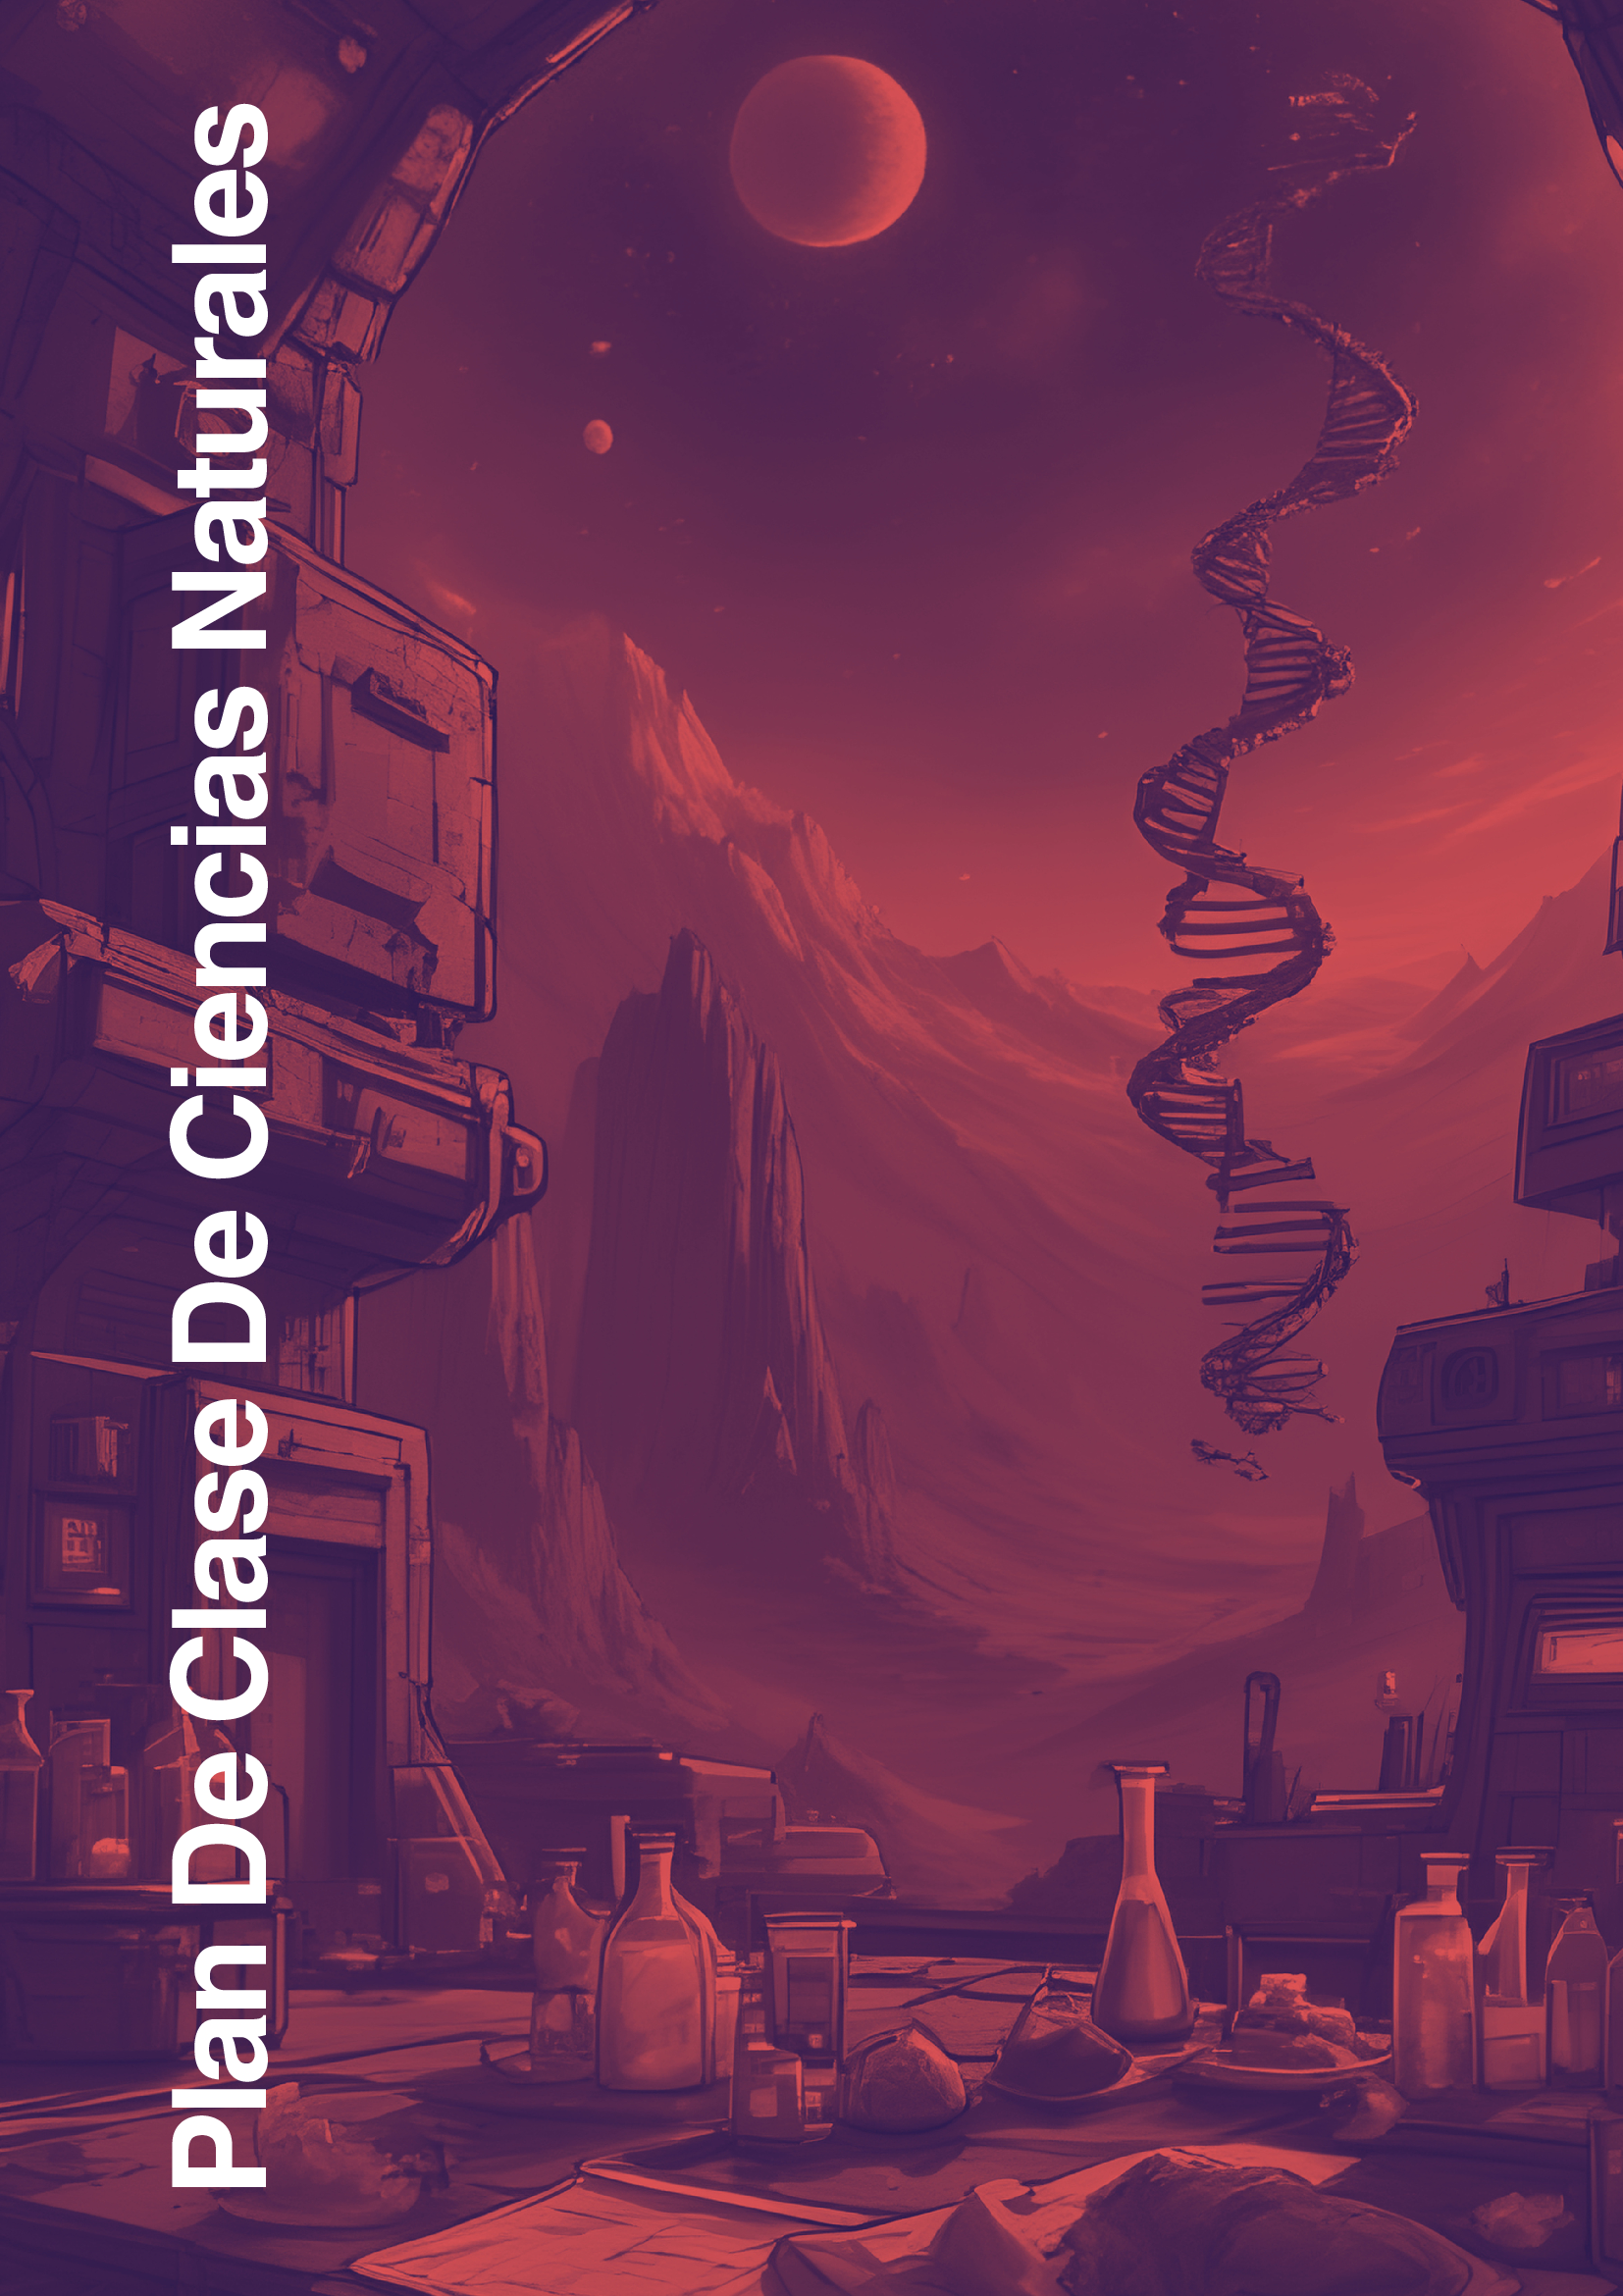
\includepdf[pages=-, fitpaper]{Portada.pdf}
  \pagenumbering{arabic}
  \pagestyle{plain}
}
\makeatletter
\@ifpackageloaded{caption}{}{\usepackage{caption}}
\AtBeginDocument{%
\ifdefined\contentsname
  \renewcommand*\contentsname{Contenido}
\else
  \newcommand\contentsname{Contenido}
\fi
\ifdefined\listfigurename
  \renewcommand*\listfigurename{Listado de Figuras}
\else
  \newcommand\listfigurename{Listado de Figuras}
\fi
\ifdefined\listtablename
  \renewcommand*\listtablename{Listado de Tablas}
\else
  \newcommand\listtablename{Listado de Tablas}
\fi
\ifdefined\figurename
  \renewcommand*\figurename{Figura}
\else
  \newcommand\figurename{Figura}
\fi
\ifdefined\tablename
  \renewcommand*\tablename{Tabla}
\else
  \newcommand\tablename{Tabla}
\fi
}
\@ifpackageloaded{float}{}{\usepackage{float}}
\floatstyle{ruled}
\@ifundefined{c@chapter}{\newfloat{codelisting}{h}{lop}}{\newfloat{codelisting}{h}{lop}[chapter]}
\floatname{codelisting}{Listado}
\newcommand*\listoflistings{\listof{codelisting}{Listado de Listados}}
\makeatother
\makeatletter
\makeatother
\makeatletter
\@ifpackageloaded{caption}{}{\usepackage{caption}}
\@ifpackageloaded{subcaption}{}{\usepackage{subcaption}}
\makeatother
\usepackage{bookmark}
\IfFileExists{xurl.sty}{\usepackage{xurl}}{} % add URL line breaks if available
\urlstyle{same}
\hypersetup{
  pdftitle={Natura Docens},
  pdflang={es},
  colorlinks=true,
  linkcolor={docere-link},
  filecolor={Maroon},
  citecolor={docere-cite},
  urlcolor={docere-url},
  pdfcreator={LaTeX via pandoc}}


\title{Natura Docens}
\author{}
\date{}
\begin{document}
\frontmatter
\maketitle

\renewcommand*\contentsname{Contenido}
{
\setcounter{tocdepth}{0}
\tableofcontents
}

\mainmatter
\chapter{Estructura del libro}\label{estructura-del-libro}

\textbf{Guía didáctica para grados 6° a 11° con enfoque pedagógico
inclusivo.}

Este libro reúne planes de clase estructurados con teoría, ideas
previas, contextualización, ejercicios, retos, aplicación y componente
socioemocional para cada tema del área de Ciencias Naturales.

Cada tema está organizado en las siguientes secciones:

\section{Detalles de la Estructura}\label{detalles-de-la-estructura}

\begin{itemize}
\tightlist
\item
  \textbf{Teoría} --- Contenido conceptual fundamental
\item
  \textbf{Ideas previas} --- Cuentos y preguntas para activar
  conocimientos
\item
  \textbf{Contextualización} --- Aplicación del método Richard Feynman
\item
  \textbf{Contextualización para caracterizados} --- Estrategias
  diferenciadas (cognitivo, TDAH, TEA, accesibilidad visual, motora)
\item
  \textbf{Ejemplo} --- Casos guiados en niveles básico, intermedio y
  avanzado
\item
  \textbf{Ejercicios} --- Práctica estructurada
\item
  \textbf{Retos} --- Problemas de profundización
\item
  \textbf{Aplicación} --- Conexión con la vida real y laboratorio
\item
  \textbf{Socioemocional} --- Acompañamiento emocional del aprendizaje
\end{itemize}

\part{Generalidades}

\chapter{Generalidades}\label{generalidades-1}

Este documento presenta un plan de temas por periodos para el
\textbf{área de Ciencias Naturales} (Biología, Física y Química),
dirigido a docentes, como guía de organización y secuenciación de
contenidos durante el año escolar.

\section{Importante -
Fundamentación}\label{importante---fundamentaciuxf3n}

En fundamentación se establece el contenido teórico específico y
concreto. Acá se establece la información respaldada por libros
universitarios, enfocada a la temática específica o artículos de
revisión o de investigación. El docente que quiera aportar en la forma
de explicar el concepto lo puede realizar en conceptualización. Este
documento se actualiza de forma colaborativa. Para facilitar el
seguimiento, se recomienda registrar aquí quién realizó cada
modificación y qué se cambió (por ejemplo: correcciones de redacción,
incorporación de secciones, ajuste de figuras o referencias).

{\def\LTcaptype{none} % do not increment counter
\begin{longtable}[]{@{}lll@{}}
\toprule\noalign{}
Fecha & Usuario & Cambio realizado \\
\midrule\noalign{}
\endhead
\bottomrule\noalign{}
\endlastfoot
8-Jun-2026 & Camilo Tayac & Reactivo Limite \\
\end{longtable}
}

\section{Prefacio}\label{prefacio}

Este libro de Ciencias Naturales está diseñado para acompañar el proceso
de aprendizaje desde grado sexto hasta grado undécimo, integrando
Biología, Física y Química en una ruta progresiva. El material prioriza
la comprensión conceptual, el razonamiento científico y la aplicación
práctica de los contenidos en contextos escolares.

La organización de cada unidad busca mantener un equilibrio entre
precisión académica y lenguaje accesible. Por esa razón, los temas se
presentan de lo general a lo específico, con explicaciones
estructuradas, ejemplos guiados y actividades que fortalecen habilidades
cognitivas como análisis, interpretación y resolución de problemas.

El enfoque metodológico combina fundamentación teórica,
contextualización didáctica y ejercicios de consolidación. De este modo,
el texto puede utilizarse tanto en clase como en trabajo autónomo,
procesos de nivelación o preparación de evaluaciones.

\section{Cómo está organizado este
libro}\label{cuxf3mo-estuxe1-organizado-este-libro}

Cada bloque por grado incluye una secuencia de contenidos por periodos
académicos y por área. Dentro de cada tema, se mantiene una estructura
consistente para facilitar la lectura:

\begin{itemize}
\tightlist
\item
  presentación del concepto central,
\item
  desarrollo explicativo paso a paso,
\item
  ejemplos de aplicación,
\item
  actividades para fortalecer la comprensión.
\end{itemize}

\section{Sugerencias de uso}\label{sugerencias-de-uso}

Se recomienda trabajar los contenidos en orden, registrar ideas clave y
verificar la comprensión con los ejercicios propuestos. Cuando aparezcan
dificultades, conviene retomar los ejemplos y relacionarlos con
situaciones del entorno cotidiano.

\chapter{Plan de Área de Ciencias
Naturales}\label{plan-de-uxe1rea-de-ciencias-naturales}

\section{Biología}\label{biologuxeda}

{\def\LTcaptype{none} % do not increment counter
\begin{longtable}[]{@{}
  >{\raggedright\arraybackslash}p{(\linewidth - 10\tabcolsep) * \real{0.1667}}
  >{\raggedright\arraybackslash}p{(\linewidth - 10\tabcolsep) * \real{0.1667}}
  >{\raggedright\arraybackslash}p{(\linewidth - 10\tabcolsep) * \real{0.1667}}
  >{\raggedright\arraybackslash}p{(\linewidth - 10\tabcolsep) * \real{0.1667}}
  >{\raggedright\arraybackslash}p{(\linewidth - 10\tabcolsep) * \real{0.1667}}
  >{\raggedright\arraybackslash}p{(\linewidth - 10\tabcolsep) * \real{0.1667}}@{}}
\toprule\noalign{}
\begin{minipage}[b]{\linewidth}\raggedright
Grado
\end{minipage} & \begin{minipage}[b]{\linewidth}\raggedright
Periodo
\end{minipage} & \begin{minipage}[b]{\linewidth}\raggedright
Eje Temático
\end{minipage} & \begin{minipage}[b]{\linewidth}\raggedright
DBA Alineado
\end{minipage} & \begin{minipage}[b]{\linewidth}\raggedright
Pre-requisito
\end{minipage} & \begin{minipage}[b]{\linewidth}\raggedright
Capítulo
\end{minipage} \\
\midrule\noalign{}
\endhead
\bottomrule\noalign{}
\endlastfoot
6° & I & Fundamentos de la Materia y la Vida & DBA 3: Clasificación de
materiales (sustancias puras y mezclas). & Conocimientos básicos sobre
la materia. & 1, 2 y 3 \\
6° & II & La Célula como Unidad Funcional & DBA 4: Funciones básicas de
la célula (transporte, energía y división). & Dominio de moléculas
biológicas (Periodo 1). & 4 y 5 \\
6° & III & Clasificación y Diversidad & DBA 5: Clasificación taxonómica
según el tipo de células y biodiversidad. & Diferenciación entre células
procariotas y eucariotas (Periodo 2). & 19, 20 y 21 \\
6° & IV & Fenómenos Físicos y Químicos & DBA 1: Cargas eléctricas. DBA
2: Influencia de T y P en propiedades fisicoquímicas. & Conceptos de
energía y transformación de la materia (Periodo 1). & 6 e integración \\
& & & & & \\
7° & I & Transformación de Energía Celular & DBA 3: Fotosíntesis como
construcción de materia y Respiración Celular. & Estructura de organelos
(cloroplastos y mitocondrias). & 7 y 8 \\
7° & II & Dinámica de Poblaciones y Nutrición & DBA 3: Nutrición
autótrofa/heterótrofa en cadenas y redes tróficas. & Conceptos de
fotosíntesis (Periodo 1). & 28 y 29 \\
7° & III & Flujo de Energía y Ciclos Nutrientes & DBA 4: Ciclos
biogeoquímicos (C, N y H₂O) y mantenimiento de suelos. & Transferencia
de energía en redes tróficas (Periodo 2). & 30 \\
7° & IV & Biodiversidad e Impacto Humano & DBA 4: Efectos de la
intervención humana (erosión, minería) y conservación. & Ciclos del agua
y carbono (Periodo 3). & 31 \\
& & & & & \\
8° & I & Reproducción Celular y Herencia & DBA 5: Importancia de la
división celular (mitosis/meiosis) en la vida. & Concepto de célula y
núcleo (Grado 6). & 9 y 10 \\
8° & II & Sistemas de Reproducción Organísmica & DBA 5: Reproducción
sexual/asexual en animales y plantas; salud y variabilidad. & Procesos
de meiosis y gametogénesis (Periodo 1). & 42 y 46 \\
8° & III & Homeostasis y Control Maestro & DBA 4: Relación entre sistema
nervioso, endocrino y la organización corporal. & Conceptos básicos de
tejidos y órganos (Grado 7). & 32, 38 y 39 \\
8° & IV & Sistemas de Ejecución, Defensa y Excreción & DBA 4: Relación
entre sistema inmune, urinario (excretor), muscular y esqueleto. &
Coordinación nerviosa y señales químicas (Periodo 3). & 36, 37 y 41 \\
& & & & & \\
9° & I & Genética Clásica y Herencia & DBA 4: Principios mendelianos y
post-mendelianos; predicción de características. & Conceptos de meiosis
y reproducción (Grado 8). & 11 \\
9° & II & Genética Molecular y Biotecnología & DBA 5: Estructura del
ADN, expresión génica (proteínas) y biotecnología. & Patrones de
herencia y variabilidad (Periodo 1). & 12, 13 y 14 \\
9° & III & Teorías de la Evolución & DBA 6: Selección natural, ancestro
común y evidencias de la evolución. & Mecanismos de mutación y cambios
en el ADN (Periodo 2). & 15, 16 y 17 \\
9° & IV & Historia de la Vida y Diversidad & DBA 6: Eras geológicas,
sistemática y conservación de la biodiversidad. & Procesos de
especiación y selección natural (Periodo 3). & 18, 19 \\
& & & & & \\
10° & I & Fundamentos Moleculares de la Biotecnología & DBA 4:
Estructura y función del ADN y ARN en la manipulación genética. &
Genética mendeliana y celular (visto en 9°). & 12 y 13 \\
10° & II & Técnicas de Ingeniería Genética & DBA 4: Descripción de
técnicas (PCR, clonación, secuenciación y edición). & Mecanismos de
expresión y regulación génica (Periodo 1). & 14 \\
10° & III & Aplicaciones en Salud y Reproducción & DBA 4: Fertilización
asistida, terapias génicas y medicina genómica. & Fisiología
reproductiva y desarrollo animal. & 14, 42 y 43 \\
10° & IV & Bioética e Impacto Socio-Ambiental & DBA 4: Implicaciones
legales, sociales y ambientales de los transgénicos. & Aplicaciones
biotecnológicas en agricultura y salud (Periodo 3). & 14 y 31 \\
& & & & & \\
11° & I & Cambio Climático y Flujo de Energía & DBA 5: Explicación del
calentamiento global, sus causas y acciones globales. & Ciclos
biogeoquímicos y flujo de energía (Grado 7). & 29 \\
11° & II & Colombia: País Megadiverso & DBA 5: Implicaciones sociales y
ambientales de la megadiversidad en Colombia. & Clasificación de
ecosistemas y biomas (Grado 4). & 30 \\
11° & III & Impacto Humano en la Biodiversidad & DBA 5: Efectos de la
minería, ganadería, agricultura y obras civiles en el país. & Análisis
de intervención humana en suelos (Grado 7). & 31 \\
11° & IV & Gestión y Conservación Ambiental & DBA 5: Diseño de
investigaciones y acciones para evitar el maltrato y tráfico ilegal. &
Visión sistémica de la biodiversidad (Periodo 2 y 3). & 31 \\
\end{longtable}
}

\section{Química}\label{quuxedmica}

{\def\LTcaptype{none} % do not increment counter
\begin{longtable}[]{@{}
  >{\raggedright\arraybackslash}p{(\linewidth - 10\tabcolsep) * \real{0.1667}}
  >{\raggedright\arraybackslash}p{(\linewidth - 10\tabcolsep) * \real{0.1667}}
  >{\raggedright\arraybackslash}p{(\linewidth - 10\tabcolsep) * \real{0.1667}}
  >{\raggedright\arraybackslash}p{(\linewidth - 10\tabcolsep) * \real{0.1667}}
  >{\raggedright\arraybackslash}p{(\linewidth - 10\tabcolsep) * \real{0.1667}}
  >{\raggedright\arraybackslash}p{(\linewidth - 10\tabcolsep) * \real{0.1667}}@{}}
\toprule\noalign{}
\begin{minipage}[b]{\linewidth}\raggedright
Grado
\end{minipage} & \begin{minipage}[b]{\linewidth}\raggedright
Periodo
\end{minipage} & \begin{minipage}[b]{\linewidth}\raggedright
Eje Temático
\end{minipage} & \begin{minipage}[b]{\linewidth}\raggedright
DBA Alineado
\end{minipage} & \begin{minipage}[b]{\linewidth}\raggedright
Pre-requisito
\end{minipage} & \begin{minipage}[b]{\linewidth}\raggedright
Capítulo
\end{minipage} \\
\midrule\noalign{}
\endhead
\bottomrule\noalign{}
\endlastfoot
6° & I & La materia y sus propiedades generales. & --- & --- & --- \\
6° & II & Clases de materia. & --- & --- & --- \\
6° & III & Mezclas y su clasificación. & --- & --- & --- \\
6° & IV & Técnicas de separación de mezclas. & --- & --- & --- \\
& & & & & \\
7° & I & Teoría atómica y estructura atómica. & --- & --- & --- \\
7° & II & Propiedades de la materia. & --- & --- & --- \\
7° & III & Propiedades fisicoquímicas. & --- & --- & --- \\
7° & IV & Cambios químicos básicos. & --- & --- & --- \\
& & & & & \\
8° & I & Estructura atómica. Modelos atómicos y Tabla periódica. & --- &
--- & --- \\
8° & II & Enlaces químicos (Iónico y Covalente). & --- & --- & --- \\
8° & III & Nomenclatura inorgánica (Óxidos, bases, ácidos). & --- & ---
& --- \\
& & & & & \\
9° & I & Mol, masa molar y estequiometría. & --- & --- & --- \\
9° & II & Soluciones y concentraciones químicas. & --- & --- & --- \\
9° & III & Leyes de los gases (Boyle, Charles, Gay-Lussac). & --- & ---
& --- \\
9° & IV & Química orgánica: Introducción al Carbono. & --- & --- &
--- \\
& & & & & \\
10° & I & Solución, disolución y ecuaciones químicas. & --- & --- &
--- \\
10° & III & Reacciones químicas y estequiometría. & --- & --- & --- \\
10° & IV & Gases ideales y estados de agregación. & --- & --- & --- \\
& & & & & \\
11° & I & Hidrocarburos (Alcanos, Alquenos, Alquinos). & --- & --- &
--- \\
11° & II & Grupos funcionales oxigenados y nitrogenados. & --- & --- &
--- \\
11° & III & Biomoléculas: Carbohidratos, lípidos y proteínas. & --- &
--- & --- \\
11° & IV & Cinética y equilibrio químico. Química ambiental. & --- & ---
& --- \\
\end{longtable}
}

\section{Física}\label{fuxedsica}

{\def\LTcaptype{none} % do not increment counter
\begin{longtable}[]{@{}
  >{\raggedright\arraybackslash}p{(\linewidth - 10\tabcolsep) * \real{0.1667}}
  >{\raggedright\arraybackslash}p{(\linewidth - 10\tabcolsep) * \real{0.1667}}
  >{\raggedright\arraybackslash}p{(\linewidth - 10\tabcolsep) * \real{0.1667}}
  >{\raggedright\arraybackslash}p{(\linewidth - 10\tabcolsep) * \real{0.1667}}
  >{\raggedright\arraybackslash}p{(\linewidth - 10\tabcolsep) * \real{0.1667}}
  >{\raggedright\arraybackslash}p{(\linewidth - 10\tabcolsep) * \real{0.1667}}@{}}
\toprule\noalign{}
\begin{minipage}[b]{\linewidth}\raggedright
Grado
\end{minipage} & \begin{minipage}[b]{\linewidth}\raggedright
Periodo
\end{minipage} & \begin{minipage}[b]{\linewidth}\raggedright
Eje Temático
\end{minipage} & \begin{minipage}[b]{\linewidth}\raggedright
DBA Alineado
\end{minipage} & \begin{minipage}[b]{\linewidth}\raggedright
Pre-requisito
\end{minipage} & \begin{minipage}[b]{\linewidth}\raggedright
Capítulo
\end{minipage} \\
\midrule\noalign{}
\endhead
\bottomrule\noalign{}
\endlastfoot
6° & I & Introducción a la física. Carga, fuerza y corriente eléctrica.
& --- & --- & --- \\
6° & II & Fuentes de voltaje, resistencia y circuitos eléctricos. & ---
& --- & --- \\
6° & III & Temperatura y densidad. Magnetismo y efectos de la corriente.
& --- & --- & --- \\
6° & IV & Electromagnetismo e inducción electromagnética. & --- & --- &
--- \\
& & & & & \\
7° & I & Movimiento, rapidez, aceleración y principio de inercia. & ---
& --- & --- \\
7° & II & Fuerza, masa y rozamiento. Peso y densidad. & --- & --- &
--- \\
7° & III & Trabajo, potencia y energía. & --- & --- & --- \\
7° & IV & Trabajo, potencia y energía (Continuación). & --- & --- &
--- \\
& & & & & \\
8° & I & Mecánica de fluidos: Densidad y presión. & --- & --- & --- \\
8° & II & Principios de Arquímedes y Pascal. & --- & --- & --- \\
8° & III & Calor y temperatura. Escalas termométricas. & --- & --- &
--- \\
8° & IV & Termodinámica y transferencia de calor. & --- & --- & --- \\
& & & & & \\
9° & I & Movimiento ondulatorio y fenómenos ondulatorios. & --- & --- &
--- \\
9° & II & Acústica: Naturaleza y cualidades del sonido. & --- & --- &
--- \\
9° & III & Óptica: Reflexión y refracción de la luz. & --- & --- &
--- \\
9° & IV & Espejos, lentes y el funcionamiento del ojo. & --- & --- &
--- \\
& & & & & \\
10° & I & Cinemática: Vectores, MRU y MRUA. & --- & --- & --- \\
10° & II & Dinámica: Leyes de Newton y fuerzas. & --- & --- & --- \\
10° & III & Trabajo, Energía y Potencia. & --- & --- & --- \\
10° & IV & Estática y mecánica de fluidos. & --- & --- & --- \\
& & & & & \\
11° & I & Movimiento Armónico Simple (MAS) y Ondas. & --- & --- & --- \\
11° & II & Sonido y Óptica geométrica. & --- & --- & --- \\
11° & III & Electrostática y Electrodinámica (Ley de Ohm). & --- & --- &
--- \\
11° & IV & Electromagnetismo y Física Moderna. & --- & --- & --- \\
\end{longtable}
}

\part{Décimo - Química}

\chapter{Reactivo límite}\label{reactivo-luxedmite}

\setcolorsection{e8e8e8}{d0d0d0}

\section{Teoría}\label{teoruxeda}

La \textbf{estequiometría} es la rama de la química que estudia las
relaciones cuantitativas entre reactivos y productos en una reacción
química balanceada. Cuando se lleva a cabo una reacción, los reactivos
no siempre están presentes en las proporciones exactas que indica la
ecuación balanceada. En tales casos, uno de los reactivos se consume
completamente antes que los demás, limitando la cantidad de producto que
se puede formar. A este reactivo se le denomina \textbf{reactivo límite}
(o reactivo limitante), mientras que los reactivos que no se consumen
totalmente reciben el nombre de \textbf{reactivos en exceso} (Chang y
Goldsby 2017).

Para identificar el reactivo límite se siguen cuatro pasos: (1) escribir
y balancear la ecuación química; (2) convertir las masas de los
reactivos a moles usando las masas molares; (3) dividir los moles de
cada reactivo entre su coeficiente estequiométrico en la ecuación
balanceada; y (4) el reactivo con el menor cociente es el reactivo
límite. Una vez identificado, se usan sus moles para calcular la
cantidad máxima de producto posible, denominada \textbf{rendimiento
teórico}.

\textbf{Fórmula (1):}

\[ n = \frac{m}{M} \tag{1} \]

Donde \(n\) = cantidad de sustancia (mol), \(m\) = masa del reactivo
(g), \(M\) = masa molar (g/mol).

El \textbf{porcentaje de rendimiento} relaciona el rendimiento real
(obtenido experimentalmente) con el rendimiento teórico:

\textbf{Fórmula (2):}

\[ \% \text{ rendimiento} = \frac{\text{rendimiento real}}{\text{rendimiento teórico}} \times 100 \tag{2} \]

Donde rendimiento real = masa de producto obtenida experimentalmente
(g), rendimiento teórico = masa máxima calculada a partir del reactivo
límite (g).

(Brown et~al. 2022)

\setcolorsection{f9ebaf}{e8d68a}

\section{Ideas Previas}\label{ideas-previas}

Imagina que estás armando emparedados para una fiesta y tienes 12
rebanadas de pan y 8 tajadas de queso. Cada emparedado necesita dos
rebanadas de pan y una tajada de queso. Empiezas a armar y, después del
octavo emparedado, te das cuenta de que ya no queda queso, pero todavía
te sobran rebanadas de pan. El queso determinó cuántos emparedados
pudiste hacer.

\begin{itemize}
\item
  \textbf{¿Qué crees que pasaría si, en lugar de 8 tajadas de queso,
  hubieras tenido 15? ¿Habrían cambiado los emparedados que lograste
  armar?}

  \(\underline{\hspace{6cm}}\)

  \(\underline{\hspace{6cm}}\)
\item
  \textbf{¿Puedes imaginar una situación similar en tu casa donde un
  ingrediente se acabe antes que otro cuando cocinas o preparas algo?}

  \(\underline{\hspace{6cm}}\)

  \(\underline{\hspace{6cm}}\)
\item
  \textbf{¿Crees que el ingrediente que ``sobra'' podría usarse para
  algo más después de terminar la receta original?}

  \(\underline{\hspace{6cm}}\)

  \(\underline{\hspace{6cm}}\)
\item
  \textbf{¿Por qué será importante identificar cuál ingrediente se acaba
  primero cuando trabajas con cantidades limitadas?}

  \(\underline{\hspace{6cm}}\)

  \(\underline{\hspace{6cm}}\)
\item
  \textbf{¿Qué crees que significa que algo sea ``limitante'' en un
  proceso cotidiano?}

  \(\underline{\hspace{6cm}}\)

  \(\underline{\hspace{6cm}}\)
\item
  \textbf{¿Has tenido que racionar algún material en un proyecto porque
  sabías que no alcanzaba para todos?}

  \(\underline{\hspace{6cm}}\)

  \(\underline{\hspace{6cm}}\)
\item
  \textbf{Si tuvieras que explicarle a un compañero qué es un reactivo
  límite usando solo objetos del salón, ¿qué usarías y cómo lo harías?}

  \(\underline{\hspace{6cm}}\)

  \(\underline{\hspace{6cm}}\)
\item
  \textbf{¿Por qué piensas que en química es importante saber cuál
  reactivo se acaba primero?}

  \(\underline{\hspace{6cm}}\)

  \(\underline{\hspace{6cm}}\)
\end{itemize}

En el municipio de Nemocón (Cundinamarca), las minas de sal han operado
durante siglos. Los mineros saben que, para extraer una tonelada de sal,
necesitan cierta cantidad de agua y cierta cantidad de energía térmica.
Si un día solo tienen suficiente carbón para calentar el agua durante la
mitad del tiempo necesario, la producción de ese día estará limitada por
el combustible, no por el agua disponible. De manera similar, en una
reacción química uno de los reactivos se agota antes y determina cuánto
producto se puede obtener.

\setcolorsection{f2c6a0}{e0b088}

\section{Contextualización --- Método
Feynman}\label{contextualizaciuxf3n-muxe9todo-feynman}

¿Alguna vez has armado un mueble de kit y te has dado cuenta de que te
faltan tornillos? Revisas la bolsa de piezas, cuentas los tornillos que
tienes, y luego miras el instructivo: cada panel frontal necesita dos
tornillos. Resulta que tienes 10 paneles pero solo 12 tornillos. Aunque
tengas los 10 paneles listos, solo podrás fijar 6 de ellos porque los
tornillos se acaban primero. Pues bien, en química ocurre exactamente lo
mismo: los tornillos son uno de los \textbf{reactivos}, los paneles son
el otro, y el \textbf{reactivo límite} son esos tornillos que determinan
cuántos muebles completos puedes armar. Pero cuidado: en química no
siempre es tan sencillo como contar piezas, porque los reactivos se
combinan en proporciones fijas según la ecuación balanceada, y hay que
usar moles (no unidades individuales) para hacer los cálculos correctos.

\setcolorsection{d6c7e7}{c0b0d8}

\section{Caracterizados --- TDAH}\label{caracterizados-tdah}

Identificar el reactivo limitante es un juego de 4 movimientos. Antes de
empezar, visualiza esto: cada molécula de CO necesita 2 moléculas de H₂
para formar metanol --- como cada sándwich necesita 2 panes. Si tienes 4
sándwiches de CO y 6 panes de H₂, ¿cuántos sándwiches completos armas?
El pan se acaba antes. Ese es el reactivo limitante. Ahora tradúcelo a
números con la ecuación: \(n_{CO} = 4\) mol y \(n_{H_2} = 6\) mol, luego
usa los coeficientes (\(1\) para CO, \(2\) para H₂) para calcular cuánto
producto da cada uno. El que da menos moles es el limitante. En el
laboratorio, esto significa que el H₂ se consume primero y la reacción
se detiene. \textbf{Movimiento 1:} anota la ecuación balanceada.
\textbf{Movimiento 2:} convierte los datos a moles. \textbf{Movimiento
3:} calcula el producto de cada reactivo usando los coeficientes.
\textbf{Movimiento 4:} el que produce menos moles es el limitante ---
márcalo con una estrella. Has ganado esta ronda.

\textbf{Ejemplo:} En
\(\text{CO} + 2\text{H}_2 \rightarrow \text{CH}_3\text{OH}\), tienes
\(4\) mol de CO y \(6\) mol de H₂. Movimiento 3: CO produce \(4\) mol de
metanol; H₂ produce \(3\) mol. Movimiento 4: el H₂ da menos → es el
limitante. \textbf{Ahora tapa el cálculo y explica en voz alta por qué
dividiste los moles de H₂ entre 2.}

\textbf{Ejercicios:} Para
\(\text{N}_2 + 3\text{H}_2 \rightarrow 2\text{NH}_3\), con \(2\) mol de
N₂ y \(6\) mol de H₂, aplica los 4 movimientos. Identifica el limitante
y márcalo en tu cuaderno. \textbf{{[}Opcional: explica en voz alta los
pasos en vez de escribirlos.{]}}

\textbf{Metacognición:} 1. Si el H₂ produce \(3\) mol de metanol y el CO
produce \(4\) mol, el limitante es el H₂. ¿Por qué el reactivo que da
MENOS producto es el que determina cuánto se forma? 2. ¿Qué pasaría si
añadieras más H₂ después de que el CO ya se consumió? ¿El limitante
seguiría siendo el mismo? 3. ¿Qué movimiento del juego se te hizo más
difícil? ¿Cómo harías ese movimiento más fácil la próxima vez?

\textbf{Opción de respuesta:} Puedes responder escribiendo, dibujando o
explicándoselo a un compañero.

\textbf{Glosario:} - \textbf{Reactivo limitante:} el reactivo que se
acaba primero, como el jugador que pierde todas sus vidas antes. -
\textbf{Exceso:} el reactivo que sobra porque el otro se terminó. -
\textbf{Coeficiente:} el número que dice cuántas moléculas de cada tipo
participan, como las piezas que necesita cada sándwich. -
\textbf{Estequiometría:} la receta del juego que relaciona las
cantidades de reactivos y productos.

\(\underline{\hspace{6cm}}\)

\setcolorsection{d6c7e7}{c0b0d8}

\section{Caracterizados --- Visual}\label{caracterizados-visual}

Observa esta relación: cada molécula de CO (1 círculo azul) necesita 2
moléculas de H₂ (2 círculos rojos) para formar 1 molécula de metanol (1
círculo verde). Con 4 círculos azules y 6 círculos rojos, los pares se
agotan cuando los círculos rojos se terminan --- cada azul gasta 2
rojos. El reactivo limitante es el que se acaba primero visualmente.
Ahora tradúcelo a números en esta tabla:

{\def\LTcaptype{none} % do not increment counter
\begin{longtable}[]{@{}lccc@{}}
\toprule\noalign{}
Reactivo & Moles & Coeficiente & Moles de metanol que produce \\
\midrule\noalign{}
\endhead
\bottomrule\noalign{}
\endlastfoot
CO (azul) & \(4\) & \(1\) & \(4 \times \frac{1}{1} = 4\) \\
H₂ (rojo) & \(6\) & \(2\) & \(6 \times \frac{1}{2} = 3\) \\
\end{longtable}
}

El H₂ (rojo) produce solo \(3\) mol de metanol → es el limitante. En el
laboratorio, el H₂ se consume primero y la reacción se detiene.
\textbf{Ahora cubre los valores de la tabla y reconstruye el diagrama de
flujo de memoria: datos → moles → producto por reactivo → limitante.}

\textbf{Ejemplo:} Para
\(2\text{Al} + \text{Fe}_2\text{O}_3 \rightarrow \text{Al}_2\text{O}_3 + 2\text{Fe}\)
con \(54\) g de Al y \(160\) g de Fe₂O₃, dibuja la proporción como
barras: Al (gris) \(2\) mol, Fe₂O₃ (café) \(1\) mol. Cada Al produce
\(1\) mol de Al₂O₃; Fe₂O₃ produce \(1\) mol. Ambos producen igual → no
hay limitante.

\textbf{Ejercicios:} Para
\(\text{N}_2 + 3\text{H}_2 \rightarrow 2\text{NH}_3\) con \(2\) mol de
N₂ y \(6\) mol de H₂, completa una tabla como la de arriba
\textbf{{[}opcional: dibuja el diagrama de barras en lugar de la
tabla{]}}.

\textbf{Metacognición:} 1. Dibuja lo que pasa a nivel de partículas
cuando el H₂ es el limitante. ¿Cómo se ven las moléculas de CO y H₂
antes y después de la reacción? 2. ¿Qué relación visual hay entre los
coeficientes de la ecuación y la altura de las barras en tu diagrama? 3.
Si el coeficiente del H₂ fuera \(3\) en vez de \(2\), ¿cómo cambiaría el
diagrama de barras?

\textbf{Opción de respuesta:} Puedes responder escribiendo, dibujando o
explicándoselo a un compañero.

\textbf{Glosario:} - \textbf{Reactivo limitante:} el reactivo cuya barra
(o círculo) se acaba primero; visualmente el que tiene menos producto. -
\textbf{Coeficiente:} el número que multiplica la altura de la barra de
cada reactivo. - \textbf{Exceso:} la parte de la barra del reactivo que
sobra, como una barra más larga que no se usó. - \textbf{Ecuación
balanceada:} el mapa visual que muestra cuántos círculos de cada color
se necesitan.

\(\underline{\hspace{6cm}}\)

\setcolorsection{d6c7e7}{c0b0d8}

\section{Caracterizados --- Dislexia}\label{caracterizados-dislexia}

Cada molecula de CO (monoxido de carbono) necesita 2 moleculas de H₂
(hidrogeno) para dar 1 molecula de CH₃OH (metanol). Esto es como una
receta: por cada 1 de CO usas 2 de H₂. Si tienes 4 de CO y 6 de H₂,
cuenta cuantas veces puedes repetir la receta. El CO da para 4 veces
(porque tienes 4 y necesitas 1 cada vez). El H₂ da para 3 veces (porque
tienes 6 y necesitas 2 cada vez). El que da para menos veces es el
limitante: el H₂. En el laboratorio, el H₂ se acaba primero. Ahora
escribe los calculos: \(4 \div 1 = 4\), \(6 \div 2 = 3\). \textbf{Ahora
tapa los pasos y dime en voz alta cual fue el primer paso: ¿que tenias
que hacer primero?}

\textbf{Ejemplo:} En
\(2\text{Al} + \text{Fe}_2\text{O}_3 \rightarrow \text{Al}_2\text{O}_3 + 2\text{Fe}\),
tienes \(54\) g de Al y \(160\) g de Fe₂O₃. Primero pasas a moles:
\(54 \div 27 = 2\) mol de Al, \(160 \div 160 = 1\) mol de Fe₂O₃. Despues
usas la receta (coeficientes): cada 2 de Al dan 1 de Al₂O₃. El Al da
\(2 \times \frac{1}{2} = 1\) mol. El Fe₂O₃ da
\(1 \times \frac{1}{1} = 1\) mol. Los dos dan igual → no hay limitante.
\textbf{Sin mirar la solucion, explicale a un amigo de 10 años como
llegaste a ese resultado.}

\textbf{Ejercicios:} Para
\(\text{N}_2 + 3\text{H}_2 \rightarrow 2\text{NH}_3\), con \(2\) mol de
N₂ y \(6\) mol de H₂, identifica el limitante. \textbf{{[}Opcional:
graba un audio explicando el procedimiento en vez de escribirlo.{]}}

\textbf{Metacognición:} 1. Sin leer la teoria otra vez, explica cual es
la relacion entre los coeficientes (los numeros grandes de la ecuacion)
y las moleculas. 2. ¿El CO da 4 y el H₂ da 3. El limitante es el H₂
porque da menos. ¿Por que el menor es el que manda? 3. ¿Hay algun paso
donde te hayas trabado? ¿Que harías para que ese paso sea mas facil la
proxima vez?

\textbf{Opción de respuesta:} Puedes responder escribiendo, grabando un
audio o explicándoselo a un compañero.

\textbf{Glosario:} - \textbf{Reactivo limitante:} el reactivo que se
acaba primero, el que da para menos veces la receta. - \textbf{Exceso:}
el reactivo que sobra porque el otro se termino. - \textbf{Mol:} una
cantidad fija de moleculas, como una docena de huevos pero mucho mas
grande. - \textbf{Coeficiente:} el numero grande que dice cuantas
moleculas de cada tipo participan en la reaccion.

\(\underline{\hspace{6cm}}\)

\setcolorsection{d6c7e7}{c0b0d8}

\section{Caracterizados --- Autismo}\label{caracterizados-autismo}

\textbf{Regla fija:} El reactivo limitante es el que produce la menor
cantidad de producto cuando se aplica la ecuacion balanceada. No es una
opinion ni una decision: es el resultado de seguir este algoritmo
exacto. A nivel de moleculas (submicro), la ecuacion
\(1\text{CO} + 2\text{H}_2 \rightarrow 1\text{CH}_3\text{OH}\) dice que
cada molecula de CO necesita exactamente 2 moleculas de H₂ para formar 1
de CH₃OH. Con 4 moleculas de CO y 6 de H₂, se forman 3 moleculas de
CH₃OH porque las moleculas de H₂ se acaban primero --- cada una de las 6
se empareja con una de CO hasta que se agotan. A nivel simbolico se
escribe: \(4 \times \frac{1}{1} = 4\), \(6 \times \frac{1}{2} = 3\). El
H₂ da \(3\) \textless{} \(4\) del CO. En el laboratorio (nivel
macroscopico), el H₂ se consume primero y la reaccion se detiene. El
resultado es el mismo siempre: el H₂ es el limitante.

ALGORITMO: 1. Identifica los reactivos y sus cantidades en moles. 2.
Para cada reactivo, calcula: moles de producto = moles del reactivo
\(\times \frac{\text{coeficiente del producto}}{\text{coeficiente del reactivo}}\).
3. Compara los resultados. El menor es el limitante. 4. Verifica que el
limitante sea correcto aplicando el paso 2 al reves.

\textbf{Ejemplo:} En
\(\text{CO} + 2\text{H}_2 \rightarrow \text{CH}_3\text{OH}\), \(4\) mol
de CO y \(6\) mol de H₂. Paso 2: CO → \(4 \times \frac{1}{1} = 4\) mol;
H₂ → \(6 \times \frac{1}{2} = 3\) mol. Paso 3: \(3 < 4\), el H₂ es el
limitante. \textbf{Ahora aplica el algoritmo al reves: si el H₂ es el
limitante, ¿cuantas moles de CO se consumen?}

\textbf{Ejercicios:} Para
\(\text{N}_2 + 3\text{H}_2 \rightarrow 2\text{NH}_3\) con \(2\) mol de
N₂ y \(6\) mol de H₂, aplica el algoritmo paso a paso. \textbf{{[}Opcion
A: resuelve por escrito. Opcion B: empareja cada paso del algoritmo con
su resultado.{]}} ¿Aplica la regla fija? SI / NO.

\textbf{Metacognición:} 1. Sin mirar el bloque, escribe la regla fija
con tus palabras. ¿Que dice sobre la relacion entre los coeficientes y
las moleculas? 2. ¿Seguiste los pasos del algoritmo en orden? ¿En que
paso tuviste duda? 3. Si las cantidades fueran \(3\) mol de N₂ y \(6\)
mol de H₂, ¿cambiaria el limitante? Aplica el algoritmo para
verificarlo.

\textbf{Opción de respuesta:} Puedes responder escribiendo, dibujando o
explicándoselo a un compañero.

\textbf{Glosario:} - \textbf{Reactivo limitante:} el reactivo que
produce la menor cantidad de producto segun el algoritmo. Se identifica
por comparacion numerica. - \textbf{Ecuacion balanceada:} una igualdad
que muestra la proporcion exacta en que se combinan los reactivos. -
\textbf{Coeficiente:} el numero entero que precede a cada formula.
Indica cuantas moleculas (o moles) participan. - \textbf{Exceso:} la
cantidad de un reactivo que sobra despues de que el limitante se consume
por completo.

\(\underline{\hspace{6cm}}\)

\setcolorsection{d6c7e7}{c0b0d8}

\section{Caracterizados --- Accesibilidad
Sensorial}\label{caracterizados-accesibilidad-sensorial}

Imagina que tienes 4 fichas rugosas (CO) y 6 fichas suaves (H₂). La
regla es: cada ficha rugosa necesita 2 fichas suaves para formar 1 ficha
de algodon (metanol). Empieza a emparejar: toma una rugosa, toma dos
suaves, juntalas. Repite hasta que ya no puedas hacer mas pares. Las
fichas suaves se acaban primero --- el H₂ es el reactivo limitante.
Ahora escucha la proporcion: ``uno a dos a uno'' (CO:H₂:metanol). En
simbolos: \(n_{CO} = 4\), \(n_{H_2} = 6\), el CO da \(4\) mol y el H₂ da
\(3\) mol. El H₂ es el limitante. En el laboratorio, el H₂ se consume
primero y puedes sentirlo porque al tocar los materiales, el recipiente
de H₂ queda vacio. \textbf{Cierra los ojos y describe en voz alta el
paso que sigue. Despues, señala con el dedo donde escribiste el
resultado.}

\textbf{Ejemplo:} Para
\(\text{CO} + 2\text{H}_2 \rightarrow \text{CH}_3\text{OH}\) con \(4\)
mol de CO y \(6\) mol de H₂: 1. \textbf{Tacto:} cuenta 4 fichas rugosas
y 6 suaves. 2. \textbf{Vista:} escribe \(n_{CO} = 4\), \(n_{H_2} = 6\).
3. \textbf{Calculo:} CO da \(4\) mol, H₂ da \(3\) mol. 4.
\textbf{Resultado:} el H₂ (textura suave) es el limitante. \textbf{Ahora
cierra los ojos y traza la formula con el dedo mientras repites los
pasos en voz alta.}

\textbf{Ejercicios:} Para
\(\text{N}_2 + 3\text{H}_2 \rightarrow 2\text{NH}_3\) con \(2\) mol de
N₂ y \(6\) mol de H₂, identifica el limitante usando fichas imaginarias
(2 de una textura, 6 de otra). \textbf{{[}Opcional: responde por voz en
vez de escribir.{]}}

\textbf{Metacognición:} 1. Describe con una imagen mental: ¿como se ve,
se oye o se siente que un reactivo se acaba? 2. Si cerraras los ojos y
solo usaras el tacto, ¿como sabrias cual reactivo es el limitante? 3. La
ecuacion dice que por cada pieza de CO necesitas 2 de H₂. Si cambiara el
2 por un 3, ¿como cambiaria la experiencia tactil de emparejar las
piezas?

\textbf{Opción de respuesta:} Puedes responder escribiendo, grabando un
audio o explicándoselo a un compañero.

\textbf{Glosario:} - \textbf{Reactivo limitante:} el material (textura,
color, sonido) que se acaba primero al emparejar las piezas de la
reaccion. - \textbf{Mol:} una cantidad especifica de un material, como
un monton de fichas de la misma textura. - \textbf{Coeficiente:} el
numero que dice cuantas piezas de cada textura se necesitan para formar
el producto. - \textbf{Exceso:} las fichas de la textura que sobraron
cuando la otra textura se termino.

\(\underline{\hspace{6cm}}\)

\setcolorsection{d6c7e7}{c0b0d8}

\section{Caracterizados ---
Socioemocional}\label{caracterizados-socioemocional}

Imagina que estas en una cooperativa de Sincelejo preparando limonada
para una fiesta. La receta dice: por cada 3 limones y 1 litro de agua,
obtienes 10 limonadas. Tienes 9 limones pero solo 2 litros de agua. El
agua es tu recurso limitante: aunque te sobren limones, solo puedes
hacer 20 limonadas porque el agua se acaba primero. En quimica pasa
igual: el reactivo limitante es el recurso que se acaba primero y
determina cuanto producto puedes obtener. No es un error ni una falta:
es una realidad de las proporciones, como en la vida. A nivel de
moleculas (submicro), imagina personas en una fila: cada persona de CO
necesita 2 personas de H₂ para formar un equipo de metanol. Cuando se
acaban las personas de H₂, no se pueden formar mas equipos. En simbolos:
\(n_{CO} = 4\), \(n_{H_2} = 6\), CO da \(4\) mol, H₂ da \(3\) mol. El H₂
es el limitante. En el laboratorio, el H₂ se consume primero.
\textbf{Antes de seguir, respira profundo 3 veces. Ya tienes esto.}

\textbf{Ejemplo:} Para
\(\text{CO} + 2\text{H}_2 \rightarrow \text{CH}_3\text{OH}\) con \(4\)
mol de CO y \(6\) mol de H₂: CO da \(4\) mol de metanol; H₂ da \(3\)
mol. El H₂ es el limitante. Es como si en la cooperativa tuvieras
recursos para 4 jarras por el CO pero solo para 3 por el H₂. El que da
menos es el que manda. \textbf{Ahora explica en voz alta el paso que
entendiste mejor. No importa si no es perfecto --- estas aprendiendo, y
cada paso cuenta.}

\textbf{Ejercicios:} Para
\(\text{N}_2 + 3\text{H}_2 \rightarrow 2\text{NH}_3\) con \(2\) mol de
N₂ y \(6\) mol de H₂, identifica el limitante. \textbf{{[}Opcional:
resuelve en pareja con un compañero.{]}} Al terminar, en una escala del
1 al 5, ¿como te sentiste al resolverlo?

\textbf{Metacognición:} 1. Explica con tus palabras y sin apuro: ¿que
relacion hay entre los coeficientes de la ecuacion y la cantidad de
moleculas que reaccionan? Si no te sale perfecto, esta bien. 2. ¿Como se
aplica el concepto de reactivo limitante a la distribucion de recursos
en tu comunidad? Piensa en un recurso que se acabe primero y limite lo
que se puede producir. 3. ¿Que estrategia usaste cuando algo se ponia
dificil? ¿Funciono?

\textbf{Opción de respuesta:} Puedes responder escribiendo, dibujando o
explicándoselo a un compañero.

\textbf{Glosario:} - \textbf{Reactivo limitante:} el recurso que se
acaba primero y determina cuanto se puede producir, como la harina en
una cocina comunitaria. - \textbf{Exceso:} el recurso que sobra porque
el otro se acabo primero. - \textbf{Estequiometria:} la proporcion justa
de recursos necesarios para producir algo, como la receta de una
cooperativa. - \textbf{Rendimiento:} la cantidad real de producto que se
obtiene dado el recurso limitante.

\(\underline{\hspace{6cm}}\)

\setcolorsection{b3d9f0}{94c4e0}

\section{Ejemplo --- Nivel Bajo}\label{ejemplo-nivel-bajo}

\textbf{Regla fija:} los reactivos se combinan en una proporción fija de
moles. El reactivo con el cociente
(\(\frac{\text{moles}}{\text{coeficiente}}\)) más pequeño se agota
primero. Ese es el reactivo límite.

\textbf{Enunciado:} La síntesis del metanol (\(CH_3OH\)) a partir de
monóxido de carbono e hidrógeno sigue la reacción:

\[CO(g) + 2H_2(g) \rightarrow CH_3OH(g)\]

Si se tienen \(4\,\text{mol}\) de CO y \(6\,\text{mol}\) de \(H_2\),
¿cuál es el reactivo límite y cuántos moles de \(CH_3OH\) se pueden
producir?

\textbf{Justificacion Teorica:} El reactivo límite se identifica
dividiendo los moles disponibles de cada reactivo entre su coeficiente
estequiométrico. El reactivo con el menor cociente es el límite.

\textbf{Ejecucion:}

\textbf{Paso 1: Dividir moles de CO entre su coeficiente} (el
coeficiente del CO es 1)

\[\frac{4 \text{ mol CO}}{1} = 4\]

\textbf{Paso 2: Dividir moles de H\(_2\) entre su coeficiente} (el
coeficiente del H\(_2\) es 2)

\[\frac{6 \text{ mol H}_2}{2} = 3\]

\textbf{Paso 3: Comparar cocientes}

\[3 < 4\]

Por lo tanto el H\(_2\) es el \textbf{reactivo límite}.

\textbf{Paso 4: Calcular moles de producto usando el reactivo límite}

\[6 \text{ mol H}_2 \times \frac{1 \text{ mol CH}_3\text{OH}}{2 \text{ mol H}_2} = 3 \text{ mol CH}_3\text{OH}\]

\textbf{Resultado:} El reactivo límite es el \(H_2\) y se producen
\(3\,\text{mol}\) de \(CH_3OH\) (Chang y Goldsby 2017).

\setcolorsection{b3d9f0}{94c4e0}

\section{Ejemplo --- Nivel Medio}\label{ejemplo-nivel-medio}

\textbf{Analogía:} Una ecuación química es una receta. Los reactivos son
los ingredientes. El producto es el resultado. La ecuación balanceada
dice cuánto necesitas de cada reactivo. El reactivo límite es el
ingrediente que se acaba primero.

\textbf{Enunciado:} La reacción entre el óxido nítrico y el oxígeno
produce dióxido de nitrógeno:

\[2NO(g) + O_2(g) \rightarrow 2NO_2(g)\]

Si se hacen reaccionar \(30.0\,\text{g}\) de \(NO\) con
\(20.0\,\text{g}\) de \(O_2\), determine el reactivo límite y la masa de
\(NO_2\) producida. Masas molares: \(NO = 30.01\,\text{g/mol}\),
\(O_2 = 32.00\,\text{g/mol}\), \(NO_2 = 46.01\,\text{g/mol}\).

\textbf{Justificacion Teorica:} Primero se convierten las masas a moles,
luego se dividen entre los coeficientes para identificar el reactivo
límite. Finalmente se usa la relación molar para calcular la masa de
producto.

\textbf{Ejecucion:}

\textbf{Paso 1: Convertir masa de NO a moles}

\[n_{NO} = \frac{30.0 \text{ g}}{30.01 \text{ g/mol}} = 1.00 \text{ mol NO}\]

\textbf{Paso 2: Convertir masa de O\(_2\) a moles}

\[n_{O_2} = \frac{20.0 \text{ g}}{32.00 \text{ g/mol}} = 0.625 \text{ mol O}_2\]

\textbf{Paso 3: Dividir cada uno entre su coeficiente}

NO (coeficiente 2):

\[\frac{1.00}{2} = 0.500\]

O\(_2\) (coeficiente 1):

\[\frac{0.625}{1} = 0.625\]

\textbf{Paso 4: Identificar reactivo límite}

\[0.500 < 0.625\]

El \textbf{NO} es el reactivo límite.

\textbf{Paso 5: Calcular masa de NO\(_2\) producida}

\[1.00 \text{ mol NO} \times \frac{2 \text{ mol NO}_2}{2 \text{ mol NO}} \times \frac{46.01 \text{ g}}{\text{mol}} = 46.01 \text{ g NO}_2\]

\textbf{Resultado:} El reactivo límite es el \(NO\) y se producen
\(46.01\,\text{g}\) de \(NO_2\) (Brown et~al. 2022).

\setcolorsection{b3d9f0}{94c4e0}

\section{Ejemplo --- Nivel Alto}\label{ejemplo-nivel-alto}

\textbf{Formato accesible:} \(CO(g) + 2H_2(g) \rightarrow CH_3OH(g)\)
(monóxido de carbono gaseoso más hidrógeno gaseoso produce metanol
gaseoso). Los coeficientes indican que \(1\) mol de CO reacciona con
\(2\) moles de \(H_2\).

\textbf{Enunciado:} La urea \([(NH_2)_2CO]\) se prepara a partir de
amoníaco y dióxido de carbono:

\[2NH_3(g) + CO_2(g) \rightarrow (NH_2)_2CO(ac) + H_2O(l)\]

En un proceso se hacen reaccionar \(637.2\,\text{g}\) de \(NH_3\) con
\(1142\,\text{g}\) de \(CO_2\). Determine: (a) el reactivo límite, (b)
la masa de urea que se formará, (c) la masa del reactivo en exceso que
queda sin reaccionar. Masas molares: \(NH_3 = 17.03\,\text{g/mol}\),
\(CO_2 = 44.01\,\text{g/mol}\), \((NH_2)_2CO = 60.06\,\text{g/mol}\).

\textbf{Justificación Teórica:} Se requieren tres etapas: identificar el
reactivo límite comparando los moles ajustados por coeficiente; calcular
la masa de producto usando el reactivo límite; y determinar cuánto del
otro reactivo se consumió para hallar el sobrante.

\textbf{Ejecución:}

\textbf{Paso 1: Convertir masas a moles}

\[n_{NH_3} = \frac{637.2 \text{ g}}{17.03 \text{ g/mol}} = 37.42 \text{ mol}\]

\[n_{CO_2} = \frac{1142 \text{ g}}{44.01 \text{ g/mol}} = 25.95 \text{ mol}\]

\textbf{Paso 2: Dividir entre coeficientes}

\[NH_3: \frac{37.42}{2} = 18.71\]

\[CO_2: \frac{25.95}{1} = 25.95\]

\textbf{Paso 3: Identificar reactivo límite}

\[18.71 < 25.95\]

El \textbf{\(NH_3\)} es el reactivo límite.

\textbf{Paso 4: Calcular masa de urea producida}

\[37.42 \text{ mol NH}_3 \times \frac{1 \text{ mol urea}}{2 \text{ mol NH}_3} \times \frac{60.06 \text{ g}}{\text{mol}} = 1123.7 \text{ g urea}\]

\textbf{Paso 5: Calcular moles de CO\(_2\) consumidos}

\[37.42 \text{ mol NH}_3 \times \frac{1 \text{ mol CO}_2}{2 \text{ mol NH}_3} = 18.71 \text{ mol CO}_2\]

\textbf{Paso 6: Calcular masa de CO\(_2\) sobrante}

\[25.95 - 18.71 = 7.24 \text{ mol CO}_2\]

\[7.24 \text{ mol} \times 44.01 \text{ g/mol} = 318.6 \text{ g CO}_2\]

\textbf{Resultado:} (a) El reactivo límite es el \(NH_3\). (b) Se
producen \(1124\,\text{g}\) de urea. (c) Quedan \(319\,\text{g}\) de
\(CO_2\) sin reaccionar. (Chang y Goldsby 2017)

\setcolorsection{b2e0d8}{98ccc4}

\section{Ejercicios --- Nivel Bajo}\label{ejercicios-nivel-bajo}

Aplica la \textbf{regla fija}: el reactivo con el cociente
(\(\frac{\text{moles}}{\text{coeficiente}}\)) más pequeño se agota
primero.

\begin{itemize}
\item
  Completar: En la reacción \(2H_2 + O_2 \rightarrow 2H_2O\), si se
  tienen \(3\,\text{mol}\) de \(H_2\) y \(2\,\text{mol}\) de \(O_2\), el
  reactivo límite es el \(\underline{\hspace{3cm}}\) porque su cociente
  de moles dividido entre coeficiente es \(\underline{\hspace{2cm}}\),
  mientras que el del otro reactivo es \(\underline{\hspace{2cm}}\).

  {\def\LTcaptype{none} % do not increment counter
  \begin{longtable}[]{@{}llll@{}}
  \toprule\noalign{}
  Reactivo & Moles & Coeficiente & Cociente \\
  \midrule\noalign{}
  \endhead
  \bottomrule\noalign{}
  \endlastfoot
  \(H_2\) & \(3\) & \(2\) & \(\underline{\hspace{1cm}}\) \\
  \(O_2\) & \(2\) & \(1\) & \(\underline{\hspace{1cm}}\) \\
  \end{longtable}
  }
\item
  V/F: El reactivo en exceso es aquel que se consume completamente
  durante la reacción. (\(\hspace{0.5cm}\))
\item
  Identificación: En la ecuación \(N_2 + 3H_2 \rightarrow 2NH_3\),
  indica cuál es el reactivo límite si se tienen \(2\,\text{mol}\) de
  \(N_2\) y \(5\,\text{mol}\) de \(H_2\).

  \(\underline{\hspace{6cm}}\)

  \(\underline{\hspace{6cm}}\)
\end{itemize}

\setcolorsection{b2e0d8}{98ccc4}

\section{Ejercicios --- Nivel Medio}\label{ejercicios-nivel-medio}

\textbf{Analogía:} Recuerda que una ecuación química es como una receta:
los reactivos son los ingredientes y el producto es el plato final. El
reactivo límite es el ingrediente que se acaba primero.

{\def\LTcaptype{none} % do not increment counter
\begin{longtable}[]{@{}
  >{\raggedright\arraybackslash}p{(\linewidth - 10\tabcolsep) * \real{0.1667}}
  >{\raggedright\arraybackslash}p{(\linewidth - 10\tabcolsep) * \real{0.1667}}
  >{\raggedright\arraybackslash}p{(\linewidth - 10\tabcolsep) * \real{0.1667}}
  >{\raggedright\arraybackslash}p{(\linewidth - 10\tabcolsep) * \real{0.1667}}
  >{\raggedright\arraybackslash}p{(\linewidth - 10\tabcolsep) * \real{0.1667}}
  >{\raggedright\arraybackslash}p{(\linewidth - 10\tabcolsep) * \real{0.1667}}@{}}
\toprule\noalign{}
\begin{minipage}[b]{\linewidth}\raggedright
Reactivo
\end{minipage} & \begin{minipage}[b]{\linewidth}\raggedright
Masa (g)
\end{minipage} & \begin{minipage}[b]{\linewidth}\raggedright
M (g/mol)
\end{minipage} & \begin{minipage}[b]{\linewidth}\raggedright
Moles
\end{minipage} & \begin{minipage}[b]{\linewidth}\raggedright
Coeficiente
\end{minipage} & \begin{minipage}[b]{\linewidth}\raggedright
Cociente
\end{minipage} \\
\midrule\noalign{}
\endhead
\bottomrule\noalign{}
\endlastfoot
\(\underline{\hspace{2cm}}\) & \(\underline{\hspace{2cm}}\) &
\(\underline{\hspace{2cm}}\) & \(\underline{\hspace{2cm}}\) &
\(\underline{\hspace{2cm}}\) & \(\underline{\hspace{2cm}}\) \\
\(\underline{\hspace{2cm}}\) & \(\underline{\hspace{2cm}}\) &
\(\underline{\hspace{2cm}}\) & \(\underline{\hspace{2cm}}\) &
\(\underline{\hspace{2cm}}\) & \(\underline{\hspace{2cm}}\) \\
\end{longtable}
}

\begin{itemize}
\item
  Respuesta corta: Se hacen reaccionar \(10.0\,\text{g}\) de \(Zn\)
  (masa molar \(65.38\,\text{g/mol}\)) con \(5.0\,\text{g}\) de \(HCl\)
  (masa molar \(36.46\,\text{g/mol}\)) según
  \(Zn + 2HCl \rightarrow ZnCl_2 + H_2\). ¿Cuál es el reactivo límite y
  cuántos gramos de \(ZnCl_2\) se producen?

  \(\underline{\hspace{6cm}}\)

  \(\underline{\hspace{6cm}}\)

  \(\underline{\hspace{6cm}}\)
\item
  Aplicación simple: En la reacción \(2Al + 3Cl_2 \rightarrow 2AlCl_3\),
  si se tienen \(54.0\,\text{g}\) de \(Al\) y \(106.5\,\text{g}\) de
  \(Cl_2\), ¿cuántos gramos de \(AlCl_3\) se pueden obtener?

  \(\underline{\hspace{6cm}}\)

  \(\underline{\hspace{6cm}}\)

  \(\underline{\hspace{6cm}}\)
\item
  Clasificación: Dados los siguientes pares de reactivos, identifica en
  cada caso cuál sería el reactivo límite sin hacer cálculos detallados,
  solo observando las proporciones: (a) \(1\,\text{mol}\) \(CH_4\) +
  \(3\,\text{mol}\) \(O_2\) en \(CH_4 + 2O_2 \rightarrow CO_2 + 2H_2O\);
  (b) \(2\,\text{mol}\) \(Fe\) + \(2\,\text{mol}\) \(O_2\) en
  \(4Fe + 3O_2 \rightarrow 2Fe_2O_3\).

  \(\underline{\hspace{6cm}}\)

  \(\underline{\hspace{6cm}}\)
\end{itemize}

\setcolorsection{b2e0d8}{98ccc4}

\section{Ejercicios --- Nivel Alto}\label{ejercicios-nivel-alto}

\textbf{Formato accesible:} Cada símbolo químico se acompaña de su
nombre para facilitar la identificación. Completa cada tabla de datos
antes de resolver.

{\def\LTcaptype{none} % do not increment counter
\begin{longtable}[]{@{}
  >{\raggedright\arraybackslash}p{(\linewidth - 12\tabcolsep) * \real{0.1429}}
  >{\raggedright\arraybackslash}p{(\linewidth - 12\tabcolsep) * \real{0.1429}}
  >{\raggedright\arraybackslash}p{(\linewidth - 12\tabcolsep) * \real{0.1429}}
  >{\raggedright\arraybackslash}p{(\linewidth - 12\tabcolsep) * \real{0.1429}}
  >{\raggedright\arraybackslash}p{(\linewidth - 12\tabcolsep) * \real{0.1429}}
  >{\raggedright\arraybackslash}p{(\linewidth - 12\tabcolsep) * \real{0.1429}}
  >{\raggedright\arraybackslash}p{(\linewidth - 12\tabcolsep) * \real{0.1429}}@{}}
\toprule\noalign{}
\begin{minipage}[b]{\linewidth}\raggedright
Sustancia
\end{minipage} & \begin{minipage}[b]{\linewidth}\raggedright
Fórmula
\end{minipage} & \begin{minipage}[b]{\linewidth}\raggedright
Masa (g)
\end{minipage} & \begin{minipage}[b]{\linewidth}\raggedright
M (g/mol)
\end{minipage} & \begin{minipage}[b]{\linewidth}\raggedright
Moles
\end{minipage} & \begin{minipage}[b]{\linewidth}\raggedright
Coeficiente
\end{minipage} & \begin{minipage}[b]{\linewidth}\raggedright
Cociente
\end{minipage} \\
\midrule\noalign{}
\endhead
\bottomrule\noalign{}
\endlastfoot
\(\underline{\hspace{2cm}}\) & \(\underline{\hspace{2cm}}\) &
\(\underline{\hspace{2cm}}\) & \(\underline{\hspace{2cm}}\) &
\(\underline{\hspace{2cm}}\) & \(\underline{\hspace{2cm}}\) &
\(\underline{\hspace{2cm}}\) \\
\(\underline{\hspace{2cm}}\) & \(\underline{\hspace{2cm}}\) &
\(\underline{\hspace{2cm}}\) & \(\underline{\hspace{2cm}}\) &
\(\underline{\hspace{2cm}}\) & \(\underline{\hspace{2cm}}\) &
\(\underline{\hspace{2cm}}\) \\
\end{longtable}
}

\begin{itemize}
\item
  Problema abierto: El etileno (\(C_2H_4\)) se puede preparar calentando
  hexano (\(C_6H_{14}\)):
  \(C_6H_{14} \rightarrow C_2H_4 + C_4H_{10} + CH_4\) (sin balancear).
  Si se calientan \(86.0\,\text{g}\) de hexano y se obtienen
  \(28.0\,\text{g}\) de etileno, calcula el rendimiento porcentual de la
  reacción. Sugerencia: primero balancea la ecuación.

  \(\underline{\hspace{6cm}}\)

  \(\underline{\hspace{6cm}}\)

  \(\underline{\hspace{6cm}}\)
\item
  Análisis de errores: Un estudiante afirma que en la reacción
  \(2Mg + O_2 \rightarrow 2MgO\), si se tienen \(48.6\,\text{g}\) de
  \(Mg\) y \(32.0\,\text{g}\) de \(O_2\), el reactivo límite es el
  \(O_2\) porque hay menos masa de oxígeno. Explica por qué esta
  conclusión es incorrecta y determina la respuesta correcta.

  \(\underline{\hspace{6cm}}\)

  \(\underline{\hspace{6cm}}\)

  \(\underline{\hspace{6cm}}\)
\end{itemize}

\setcolorsection{f6d5a8}{e8c490}

\section{Retos}\label{retos}

El concepto de reactivo límite se aplica en la industria farmacéutica
para maximizar la producción de medicamentos usando el principio del
reactivo más costoso como límite. Para este reto:

\begin{itemize}
\tightlist
\item
  Diseña un cartel informativo que explique los cuatro pasos para
  determinar el reactivo límite usando como ejemplo una reacción de tu
  elección. Incluye los cálculos paso a paso.
\item
  Construye un modelo físico con materiales reciclables (tapas, fichas,
  cuentas) que represente los moles de cada reactivo antes y después de
  la reacción, mostrando claramente cuál es el reactivo límite y cuál
  está en exceso.
\item
  Prepara una breve exposición (máximo 3 minutos) explicando por qué es
  importante identificar el reactivo límite en procesos industriales
  como la producción de fertilizantes o medicamentos.
\end{itemize}

\setcolorsection{c5e8d8}{a8d4c4}

\section{Aplicación --- Vida real}\label{aplicaciuxf3n-vida-real}

En la producción industrial de ácido sulfúrico (\(H_2SO_4\)) en plantas
como la de Cartagena (Colombia), el azufre se quema para formar
\(SO_2\), que luego se oxida a \(SO_3\) y finalmente se hidrata. Los
ingenieros controlan cuidadosamente las cantidades de reactivos para
garantizar que el azufre (el reactivo más costoso y menos abundante) se
consuma por completo, mientras que el oxígeno del aire se suministra en
exceso. Así se maximiza el rendimiento económico del proceso. La próxima
vez que veas una batería de carro o un producto de limpieza, recuerda
que el ácido sulfúrico que contienen se fabricó aplicando el concepto de
reactivo límite para optimizar su producción.

\setcolorsection{c5e8d8}{a8d4c4}

\section{Aplicación --- Laboratorio}\label{aplicaciuxf3n-laboratorio}

\textbf{Objetivo:} Determinar experimentalmente el reactivo límite en la
reacción entre bicarbonato de sodio y vinagre.

\textbf{Materiales:} - Bicarbonato de sodio (\(NaHCO_3\)) - Vinagre
blanco (solución de ácido acético \(CH_3COOH\) al \(5\%\)) - Balanza
digital - \(2\) vasos desechables pequeños - Cuchara plástica

\textbf{Procedimiento:}

\emph{Preparación:} 1. Pesa \(5.0\,\text{g}\) de bicarbonato de sodio
(\(NaHCO_3\)) en la balanza digital y colócalos en el vaso 1. 2. Mide
\(30\,\text{mL}\) de vinagre (\(CH_3COOH\) al \(5\%\)) con la probeta y
viértelos en el vaso 2.

\emph{Ensayo 1 --- vinagre en exceso:} 3. Vierte el vinagre del vaso 2
sobre el bicarbonato del vaso 1. Observa la efervescencia. 4. Espera a
que la reacción se detenga por completo (sin burbujas). 5. Revisa el
fondo del vaso con la cuchara: ¿quedó bicarbonato sin reaccionar? 6.
Registra en la tabla si sobró bicarbonato.

\emph{Ensayo 2 --- bicarbonato en exceso:} 7. Repite la preparación con
cantidades invertidas: \(30\,\text{g}\) de bicarbonato en el vaso 1 y
\(5\,\text{mL}\) de vinagre en el vaso 2. 8. Vierte el vinagre sobre el
bicarbonato y observa. 9. Al detenerse la reacción, verifica con la
cuchara si quedó bicarbonato sin reaccionar. 10. Compara los resultados
de ambos ensayos: ¿en cuál sobró bicarbonato? ¿Cuál fue el reactivo
límite en cada caso?

\textbf{Resultados:}

{\def\LTcaptype{none} % do not increment counter
\begin{longtable}[]{@{}
  >{\raggedright\arraybackslash}p{(\linewidth - 8\tabcolsep) * \real{0.2000}}
  >{\raggedright\arraybackslash}p{(\linewidth - 8\tabcolsep) * \real{0.2000}}
  >{\raggedright\arraybackslash}p{(\linewidth - 8\tabcolsep) * \real{0.2000}}
  >{\raggedright\arraybackslash}p{(\linewidth - 8\tabcolsep) * \real{0.2000}}
  >{\raggedright\arraybackslash}p{(\linewidth - 8\tabcolsep) * \real{0.2000}}@{}}
\toprule\noalign{}
\begin{minipage}[b]{\linewidth}\raggedright
Ensayo
\end{minipage} & \begin{minipage}[b]{\linewidth}\raggedright
\(NaHCO_3\) (g)
\end{minipage} & \begin{minipage}[b]{\linewidth}\raggedright
Vinagre (mL)
\end{minipage} & \begin{minipage}[b]{\linewidth}\raggedright
¿Sobró bicarbonato?
\end{minipage} & \begin{minipage}[b]{\linewidth}\raggedright
Reactivo límite
\end{minipage} \\
\midrule\noalign{}
\endhead
\bottomrule\noalign{}
\endlastfoot
\(1\) & \(5.0\) & \(30\) & & \\
\(2\) & \(30\) & \(5\) & & \\
\end{longtable}
}

\textbf{Conclusión:} Basado en tus observaciones, ¿qué ensayo tuvo el
vinagre como reactivo límite? ¿Cómo lo sabes?

\(\underline{\hspace{6cm}}\)

\(\underline{\hspace{6cm}}\)

\(\underline{\hspace{6cm}}\)

\setcolorsection{f0c4b8}{dcb0a4}

\section{Evaluación --- Tipo ICFES}\label{evaluaciuxf3n-tipo-icfes}

\textbf{Pregunta 1 --- Nivel Bajo}

En la reacción \(N_2 + 3H_2 \rightarrow 2NH_3\), un estudiante dispone
de \(2\,\text{mol}\) de \(N_2\) y \(4\,\text{mol}\) de \(H_2\).

De acuerdo con la información anterior, ¿cuál de las siguientes
afirmaciones es correcta?

:--- \textbar{} :--- \textbar{}\\
A. El N\(_2\) es el reactivo límite porque su coeficiente
estequiométrico es \(1\). \textbar{} B. El H\(_2\) es el reactivo límite
porque \(\frac{4}{3} < \frac{2}{1}\). \textbar{}\\
C. El N\(_2\) y el H\(_2\) están en proporción estequiométrica exacta.
\textbar{} D. El H\(_2\) es el reactivo límite porque hay menos moles de
H\(_2\) que de N\(_2\). \textbar{}

\begin{center}\rule{0.5\linewidth}{0.5pt}\end{center}

\textbf{Pregunta 2 --- Nivel Bajo}

La ecuación \(2H_2 + O_2 \rightarrow 2H_2O\) representa la formación de
agua.

Si se tienen \(4\,\text{g}\) de \(H_2\) y \(32\,\text{g}\) de \(O_2\),
¿cuál de las siguientes opciones describe correctamente la situación?
(Masas molares: \(H_2 = 2\,\text{g/mol}\), \(O_2 = 32\,\text{g/mol}\))

:--- \textbar{} :--- \textbar{}\\
A. El oxígeno es el reactivo límite porque \(32\,\text{g}\)
\(> 4\,\text{g}\). \textbar{} B. El hidrógeno es el reactivo límite
porque \(\frac{2}{2} = 1\) y \(\frac{1}{1} = 1\), están en proporción
exacta. \textbar{}\\
C. El oxígeno es el reactivo límite porque \(\frac{1}{1} = 1\) y
\(\frac{2}{2} = 1\), ambos están igual. \textbar{} D. No hay reactivo
límite porque ambos están en la proporción estequiométrica correcta.
\textbar{}

\begin{center}\rule{0.5\linewidth}{0.5pt}\end{center}

\textbf{Pregunta 3 --- Nivel Medio}

En un laboratorio se hacen reaccionar \(10.0\,\text{g}\) de calcio
(\(Ca\)) con \(10.0\,\text{g}\) de oxígeno (\(O_2\)) según la ecuación
\(2Ca + O_2 \rightarrow 2CaO\) (masas molares:
\(Ca = 40.08\,\text{g/mol}\), \(O_2 = 32.00\,\text{g/mol}\),
\(CaO = 56.08\,\text{g/mol}\)).

¿Cuál es la masa máxima de CaO que se puede obtener?

:--- \textbar{} :--- \textbar{}\\
A. \(7.0\) g \textbar{} B. \(14.0\) g \textbar{}\\
C. \(20.0\) g \textbar{} D. \(28.0\) g \textbar{}

\begin{center}\rule{0.5\linewidth}{0.5pt}\end{center}

\textbf{Pregunta 4 --- Nivel Medio}

La fermentación de la glucosa produce etanol y dióxido de carbono:
\(C_6H_{12}O_6 \rightarrow 2C_2H_5OH + 2CO_2\). Un ingeniero dispone de
\(500\,\text{g}\) de glucosa y obtiene \(200\,\text{g}\) de etanol
(masas molares: glucosa \(= 180.16\,\text{g/mol}\), etanol
\(= 46.07\,\text{g/mol}\)).

¿Cuál es el rendimiento porcentual de la reacción?

:--- \textbar{} :--- \textbar{}\\
A. \(39.1\%\) \textbar{} B. \(68.5\%\) \textbar{}\\
C. \(78.3\%\) \textbar{} D. \(100\%\) \textbar{}

\begin{center}\rule{0.5\linewidth}{0.5pt}\end{center}

\textbf{Pregunta 5 --- Nivel Alto}

En la tostación de la pirita (\(FeS_2\)) para producir \(SO_2\), la
ecuación es \(4FeS_2 + 11O_2 \rightarrow 2Fe_2O_3 + 8SO_2\). Un mineral
contiene \(240\,\text{g}\) de \(FeS_2\) con impurezas inertes y se usa
oxígeno en exceso, obteniéndose \(192\,\text{g}\) de \(SO_2\) (masas
molares: \(FeS_2 = 119.98\,\text{g/mol}\),
\(SO_2 = 64.06\,\text{g/mol}\)).

¿Cuál es el porcentaje de pureza del mineral?

:--- \textbar{} :--- \textbar{}\\
A. \(50.0\%\) \textbar{} B. \(62.5\%\) \textbar{}\\
C. \(75.0\%\) \textbar{} D. \(87.5\%\) \textbar{}

\textbf{Autoevaluación:} Reflexiona sobre tu desempeño en esta
evaluación. ¿En qué nivel te sentiste más seguro? ¿Qué concepto
necesitas repasar?

\setcolorsection{f0c4b8}{dcb0a4}

\section{Socialización}\label{socializaciuxf3n}

\textbf{Pregunta 1} --- Nivel Bajo \emph{Competencia:} Interpretación
\emph{Afirmación:} Comprende las relaciones estequiométricas en una
ecuación química balanceada. \emph{Evidencia:} Identifica correctamente
el reactivo límite dividiendo los moles disponibles entre los
coeficientes estequiométricos. \emph{Respuesta correcta:} B
\emph{Explicación:} El cociente para \(N_2\) es \(\frac{2}{1} = 2\), y
para \(H_2\) es \(\frac{4}{3} \approx 1.33\). Como \(1.33 < 2\), el
\(H_2\) es el reactivo límite.

\textbf{Pregunta 2} --- Nivel Bajo \emph{Competencia:} Argumentación
\emph{Afirmación:} Justifica la identificación del reactivo límite
basándose en cálculos estequiométricos. \emph{Evidencia:} Reconoce que
cuando los cocientes \(\frac{\text{moles}}{\text{coeficiente}}\) son
iguales, los reactivos están en proporción estequiométrica exacta y no
hay reactivo límite. \emph{Respuesta correcta:} D \emph{Explicación:}
\(H_2: \frac{2 \text{ mol}}{2} = 1\);
\(O_2: \frac{1 \text{ mol}}{1} = 1\). Al ser iguales, ambos reactivos se
consumen completamente y no hay reactivo límite.

\textbf{Pregunta 3} --- Nivel Medio \emph{Competencia:} Interpretación
\emph{Afirmación:} Determina la cantidad de producto a partir del
reactivo límite. \emph{Evidencia:} Calcula los moles de cada reactivo y
del producto usando relaciones estequiométricas. \emph{Respuesta
correcta:} B \emph{Explicación:}
\(Ca: \frac{10.0}{40.08} = 0.249\,\text{mol}\), cociente
\(= \frac{0.249}{2} = 0.1245\).
\(O_2: \frac{10.0}{32.00} = 0.3125\,\text{mol}\), cociente
\(= \frac{0.3125}{1} = 0.3125\). El Ca es el reactivo límite. Masa de
\(CaO = 0.249 \text{ mol} \times (\frac{2}{2}) \times 56.08 \text{ g/mol} = 14.0\,\text{g}\).

\textbf{Pregunta 4} --- Nivel Medio \emph{Competencia:} Argumentación
\emph{Afirmación:} Calcula el rendimiento porcentual de una reacción.
\emph{Evidencia:} Relaciona el rendimiento real con el rendimiento
teórico usando la fórmula del porcentaje de rendimiento. \emph{Respuesta
correcta:} C \emph{Explicación:} Moles de glucosa
\(= \frac{500}{180.16} = 2.775\,\text{mol}\). Rendimiento teórico de
etanol \(= 2.775 \times 2 \times 46.07 = 255.6\,\text{g}\). \(\%\)
rendimiento \(= (\frac{200}{255.6}) \times 100 = 78.3\%\).

\textbf{Pregunta 5} --- Nivel Alto \emph{Competencia:} Proposición
\emph{Afirmación:} Propone estrategias para determinar la pureza de un
mineral a partir de datos experimentales. \emph{Evidencia:} Relaciona la
masa de producto obtenida con la masa del reactivo puro necesaria,
usando la estequiometría de la reacción. \emph{Respuesta correcta:} C
\emph{Explicación:} Moles de \(SO_2\)
\(= \frac{192}{64.06} = 3.0\,\text{mol}\). Moles de \(FeS_2\) puro
\(= 3.0 \times (\frac{4}{8}) = 1.5\,\text{mol}\). Masa de \(FeS_2\) puro
\(= 1.5 \times 119.98 = 180\,\text{g}\). Pureza
\(= (\frac{180}{240}) \times 100 = 75\%\).

\setcolorsection{f4c8d8}{e0b0c4}

\section{Socioemocional}\label{socioemocional}

Al aprender sobre el reactivo límite, es normal sentir que hay muchos
pasos y cálculos que recordar. La clave está en la \textbf{Regulación
Emocional} (Ley 2503 de 2025): reconocer que la frustración inicial es
parte del proceso de aprendizaje y que cada paso resuelto es un logro.
Identificar el reactivo límite en química es como identificar aquello
que nos limita en la vida: cuando sabemos qué nos está frenando, podemos
concentrar nuestros esfuerzos en eso y avanzar. Tú ya has superado
conceptos difíciles antes; este es solo un escalón más. Respira,
organiza tus pasos como organizas los cálculos, y verás que el resultado
llega.

\chapter{Escritura de ecuaciones
químicas}\label{escritura-de-ecuaciones-quuxedmicas}

\setcolorsection{e8e8e8}{d0d0d0}

\section{Teoría}\label{teoruxeda-1}

La \textbf{ecuación química} (representación simbólica de una reacción
química) utiliza símbolos químicos para mostrar qué sucede durante un
cambio químico. En ella, las sustancias iniciales llamadas
\textbf{reactivos} (sustancias que reaccionan) se escriben a la
izquierda, y las nuevas sustancias llamadas \textbf{productos}
(sustancias producidas) se escriben a la derecha, separadas por una
flecha que indica la dirección de la reacción (Chang y Goldsby 2017).
Para que se cumpla la \textbf{ley de la conservación de la masa}
(principio de que los átomos no se crean ni se destruyen, solo se
reordenan), una ecuación debe estar balanceada. El \textbf{balanceo}
(proceso de igualar el número de átomos de cada elemento en ambos lados
de la ecuación) se realiza colocando \textbf{coeficientes
estequiométricos} (números enteros delante de las fórmulas) sin alterar
nunca los subíndices, ya que cambiarlos modificaría la identidad de las
sustancias (Brown et~al. 2022).

Para proporcionar información adicional, se indica el estado físico de
los componentes mediante subíndices abreviados en paréntesis: sólido
\((s)\), líquido \((l)\), gaseoso \((g)\) y acuoso \((ac)\) para
sustancias disueltas en agua. Un ejemplo de ecuación química balanceada
es la combustión de hidrógeno gaseoso para producir agua líquida:

\textbf{Fórmula (1):}

\[2H_2(g) + O_2(g) \rightarrow 2H_2O(l)\tag{1}\]

Donde los coeficientes indican que \(2\) moles de \(H_2\) gaseoso
reaccionan con \(1\) mol de \(O_2\) gaseoso para producir \(2\) moles de
\(H_2O\) líquida (Oriakhi 2021).

\textbf{Teoría de balanceo en pasos:} 1. \textbf{Identificar reactivos y
productos.} Escribir sus fórmulas. Colocar reactivos a la izquierda y
productos a la derecha. 2. \textbf{Contar átomos.} Contar la cantidad de
átomos de cada elemento en ambos lados. 3. \textbf{Ajustar
coeficientes.} Colocar números enteros delante de las fórmulas para
igualar los átomos. No cambiar los subíndices. 4. \textbf{Verificar
balanceo.} Confirmar que el número total de átomos es igual en reactivos
y productos.

\setcolorsection{f9ebaf}{e8d68a}

\section{Ideas Previas}\label{ideas-previas-1}

Imagina que trabajas en un taller en Bogotá armando bicicletas. Tienes
en tu mesa \(8\) llantas, \(3\) marcos y \(6\) pedales. Para armar una
bicicleta completa necesitas exactamente \(2\) llantas, \(1\) marco y
\(2\) pedales. Empiezas a ensamblar las bicicletas una por una hasta que
te das cuenta de que algunas piezas se agotan antes que otras y no
puedes seguir armando más bicicletas completas, sobrando algunas partes
sueltas.

\begin{itemize}
\item
  ¿Te ha pasado algo similar al intentar armar o construir un objeto en
  tu casa?

  \[\underline{\hspace{6cm}}\]

  \[\underline{\hspace{6cm}}\]
\item
  ¿Qué crees que pasaría si en el cuento tuvieras \(10\) llantas pero
  siguieras teniendo solo \(3\) marcos?

  \[\underline{\hspace{6cm}}\]

  \[\underline{\hspace{6cm}}\]
\item
  ¿Qué diferencia hay entre tener las piezas sueltas en el taller y
  tener la bicicleta completamente armada y funcional?

  \[\underline{\hspace{6cm}}\]

  \[\underline{\hspace{6cm}}\]
\item
  ¿Por qué crees que es importante saber la cantidad exacta de cada
  pieza antes de iniciar el proceso de ensamble?

  \[\underline{\hspace{6cm}}\]

  \[\underline{\hspace{6cm}}\]
\item
  ¿Qué sabes sobre cómo representan los científicos los cambios que
  ocurren en la naturaleza?

  \[\underline{\hspace{6cm}}\]

  \[\underline{\hspace{6cm}}\]
\item
  ¿Has visto o vivido alguna vez una situación donde una sustancia
  cambie por completo, como cuando se quema un papel o se oxida un
  clavo?

  \[\underline{\hspace{6cm}}\]

  \[\underline{\hspace{6cm}}\]
\item
  ¿Cómo crees que funcionaría una receta para preparar un pastel si
  decides cambiar la cantidad de harina sin ajustar los demás
  ingredientes?

  \[\underline{\hspace{6cm}}\]

  \[\underline{\hspace{6cm}}\]
\item
  ¿Qué te gustaría descubrir acerca de los códigos, fórmulas y símbolos
  que utilizan los químicos en sus laboratorios?

  \[\underline{\hspace{6cm}}\]

  \[\underline{\hspace{6cm}}\]
\end{itemize}

En una panadería tradicional de Cali, don José prepara pan de bono. Para
lograr la consistencia perfecta, él mezcla almidón de yuca, queso
costeño, huevo y leche en proporciones muy precisas que ha anotado en su
cuaderno. Si cambia la cantidad de un solo ingrediente, la masa no
hornea correctamente y se pierde el producto. Lo que acabas de observar
en la cocina es precisamente lo que estudiaremos hoy al analizar cómo
las sustancias se combinan en la naturaleza respetando proporciones
fijas en una reacción química.

\setcolorsection{f2c6a0}{e0b088}

\section{Contextualización --- Método
Feynman}\label{contextualizaciuxf3n-muxe9todo-feynman-1}

Explicar cómo escribir y balancear una ecuación química es como
organizar las fichas de un juego de construcción de figuras. Imagina que
tienes fichas rojas y azules sueltas. Si unes dos fichas rojas con una
azul para formar una nave de juguete, al final de la construcción debes
tener exactamente el mismo número de fichas rojas y azules con las que
iniciaste, solo que ahora están acopladas de una forma diferente. En
este juego, las fichas sueltas representan las sustancias que reaccionan
y la nave armada representa la nueva sustancia producida. El balanceo de
la ecuación consiste en colocar números grandes al inicio de cada grupo
de fichas para asegurarnos de que ninguna ficha aparezca de la nada ni
desaparezca misteriosamente en el proceso. Cuidado: esta analogía sirve
para entender la conservación de las partes, pero los átomos reales no
son piezas de plástico que se unen a presión, sino partículas que
comparten electrones debido a fuerzas de atracción invisibles.

\setcolorsection{d6c7e7}{c0b0d8}

\section{Contextualización --- Apoyo Cognitivo y
TDAH}\label{contextualizaciuxf3n-apoyo-cognitivo-y-tdah}

Este enfoque estructura el balanceo en pasos secuenciales claros y
explícitos. Reduce la carga cognitiva al fragmentar el proceso en
instrucciones directas, con énfasis en la repetición del algoritmo.
Ideal para estudiantes que necesitan rutinas predecibles y pasos bien
definidos.

\textbf{Teoría de balanceo en pasos:} 1. \textbf{Identificar reactivos y
productos.} Escribir sus fórmulas. Colocar reactivos a la izquierda y
productos a la derecha. 2. \textbf{Contar átomos.} Contar la cantidad de
átomos de cada elemento en ambos lados. 3. \textbf{Ajustar
coeficientes.} Colocar números enteros delante de las fórmulas para
igualar los átomos. No cambiar los subíndices. 4. \textbf{Verificar
balanceo.} Confirmar que el número total de átomos es igual en reactivos
y productos.

\setcolorsection{d6c7e7}{c0b0d8}

\section{Contextualización ---
Visual}\label{contextualizaciuxf3n-visual}

Este enfoque organiza los datos en tablas de conteo con codificación
cromática (coeficientes en azul, subíndices en negro). Transforma el
balanceo abstracto en tablas visuales que permiten seguir la relación
entre reactivos y productos elemento por elemento.

\textbf{Teoría visual de balanceo:}

{\def\LTcaptype{none} % do not increment counter
\begin{longtable}[]{@{}
  >{\raggedright\arraybackslash}p{(\linewidth - 6\tabcolsep) * \real{0.2500}}
  >{\raggedright\arraybackslash}p{(\linewidth - 6\tabcolsep) * \real{0.2500}}
  >{\raggedright\arraybackslash}p{(\linewidth - 6\tabcolsep) * \real{0.2500}}
  >{\raggedright\arraybackslash}p{(\linewidth - 6\tabcolsep) * \real{0.2500}}@{}}
\toprule\noalign{}
\begin{minipage}[b]{\linewidth}\raggedright
Reactivos (izquierda)
\end{minipage} & \begin{minipage}[b]{\linewidth}\raggedright
Flecha de cambio
\end{minipage} & \begin{minipage}[b]{\linewidth}\raggedright
Productos (derecha)
\end{minipage} & \begin{minipage}[b]{\linewidth}\raggedright
Regla del color
\end{minipage} \\
\midrule\noalign{}
\endhead
\bottomrule\noalign{}
\endlastfoot
Sustancias iniciales & Indica que se \textbf{(rojo)} produce & Nuevas
sustancias & Coeficientes en \textbf{(azul)} cambian moles \\
Coeficientes en \textbf{(verde)} indican cantidad & \(\rightarrow\) &
Subíndices en \textbf{(negro)} son fijos & No alterar subíndices \\
\end{longtable}
}

\textbf{Ejemplo con tabla de conteo:} Balancear la combustión de metano
(\(CH_4\)) para producir dióxido de carbono (\(CO_2\)) y agua
(\(H_2O\)): \[CH_4(g) + O_2(g) \rightarrow CO_2(g) + H_2O(g)\]

{\def\LTcaptype{none} % do not increment counter
\begin{longtable}[]{@{}
  >{\raggedright\arraybackslash}p{(\linewidth - 6\tabcolsep) * \real{0.2500}}
  >{\raggedright\arraybackslash}p{(\linewidth - 6\tabcolsep) * \real{0.2500}}
  >{\raggedright\arraybackslash}p{(\linewidth - 6\tabcolsep) * \real{0.2500}}
  >{\raggedright\arraybackslash}p{(\linewidth - 6\tabcolsep) * \real{0.2500}}@{}}
\toprule\noalign{}
\begin{minipage}[b]{\linewidth}\raggedright
Elemento
\end{minipage} & \begin{minipage}[b]{\linewidth}\raggedright
Reactivos
\end{minipage} & \begin{minipage}[b]{\linewidth}\raggedright
Productos
\end{minipage} & \begin{minipage}[b]{\linewidth}\raggedright
Estado
\end{minipage} \\
\midrule\noalign{}
\endhead
\bottomrule\noalign{}
\endlastfoot
Carbono (\(C\)) & \(1\) & \(1\) & Balanceado \\
Hidrógeno (\(H\)) & \(4\) & \(2\) & Desbalanceado \\
Oxígeno (\(O\)) & \(2\) & \(3\) (de \(2\) en \(CO_2\) + \(1\) en
\(H_2O\)) & Desbalanceado \\
\end{longtable}
}

Ajustar \(H\) colocando un coeficiente \(2\) \textbf{(azul)} en \(H_2O\)
→ Ajustar \(O\) colocando un coeficiente \(2\) \textbf{(verde)} en
\(O_2\): \[CH_4(g) + 2O_2(g) \rightarrow CO_2(g) + 2H_2O(g)\]

{\def\LTcaptype{none} % do not increment counter
\begin{longtable}[]{@{}llll@{}}
\toprule\noalign{}
Elemento & Reactivos & Productos & Estado \\
\midrule\noalign{}
\endhead
\bottomrule\noalign{}
\endlastfoot
Carbono (\(C\)) & \(1\) & \(1\) & Balanceado \\
Hidrógeno (\(H\)) & \(4\) & \(2 \times 2 = 4\) & Balanceado \\
Oxígeno (\(O\)) & \(2 \times 2 = 4\) & \(2\) + \(2 = 4\) & Balanceado \\
\end{longtable}
}

El resultado final está balanceado.

\setcolorsection{d6c7e7}{c0b0d8}

\section{Contextualización --- Dislexia y Dificultades
Lectoras}\label{contextualizaciuxf3n-dislexia-y-dificultades-lectoras}

Este enfoque utiliza lenguaje sencillo, oraciones cortas y vocabulario
cotidiano. Prioriza la comprensión del proceso sobre la terminología
técnica. Cada idea se expresa en una línea independiente para minimizar
la carga textual.

\textbf{Teoría de balanceo simple:} - El hidrógeno (\(H\)) y el oxígeno
(\(O\)) reaccionan. - Ellos forman agua (\(H_2O\)). - Los átomos se
conservan siempre. - Tú no cambias los subíndices. - Tú colocas los
coeficientes grandes. - Los coeficientes igualan los átomos.

\setcolorsection{d6c7e7}{c0b0d8}

\section{Contextualización --- Autismo y Pensamiento
Concreto}\label{contextualizaciuxf3n-autismo-y-pensamiento-concreto}

Este enfoque presenta el balanceo como una regla fija e invariable. Cada
paso sigue una secuencia lógica inquebrantable, sin ambigüedades ni
metáforas. Proporciona un algoritmo explícito que el estudiante puede
aplicar mecánicamente a cualquier ecuación.

\textbf{Regla fija:} El número total de átomos de cada elemento químico
antes de la reacción química debe ser exactamente igual al número total
de átomos después de la reacción química. No se debe modificar ningún
subíndice. Solo se deben modificar los coeficientes multiplicadores
colocados delante de las fórmulas químicas.

\setcolorsection{d6c7e7}{c0b0d8}

\section{Contextualización --- Accesibilidad
Sensorial}\label{contextualizaciuxf3n-accesibilidad-sensorial}

Este enfoque acompaña cada símbolo químico con su nombre completo y
descripción textual. Cada operación se desglosa en pasos independientes
con etiquetas claras. Reduce la abstracción al nombrar explícitamente
cada sustancia.

\textbf{Estructura accesible de balanceo:} Las ecuaciones químicas
describen reacciones. Los reactivos están a la izquierda y los productos
a la derecha. El balanceo asegura que la materia se conserve.

\setcolorsection{d6c7e7}{c0b0d8}

\section{Contextualización --- Socioemocional y
Psicosocial}\label{contextualizaciuxf3n-socioemocional-y-psicosocial}

Este enfoque enmarca el aprendizaje en un tono alentador y de
acompañamiento. Normaliza la dificultad inicial y celebra cada balanceo
completado como un logro. Integra principios de regulación emocional
para reducir la ansiedad.

Al aprender a balancear ecuaciones químicas, es muy común cometer
errores en los conteos de átomos o sentirse abrumado por intentar
diferentes combinaciones. Esta reflexión aporta a tu competencia de
\textbf{Autonomía} al recordarte que el error es una parte valiosa del
proceso científico y que tu capacidad para resolver problemas complejos
se fortalece con cada intento fallido.

\setcolorsection{b3d9f0}{94c4e0}

\section{Ejemplo --- Nivel Bajo}\label{ejemplo-nivel-bajo-1}

\textbf{Regla fija:} El número total de átomos de cada elemento químico
antes de la reacción química debe ser exactamente igual al número total
de átomos después de la reacción química. No se modifica ningún
subíndice. Solo se modifican los coeficientes.

\textbf{Enunciado:} Balancear la ecuación química para la combustión de
hidrógeno gaseoso (\(H_2\)) en presencia de oxígeno (\(O_2\)) para
producir agua líquida (\(H_2O\)):
\[H_2(g) + O_2(g) \rightarrow H_2O(l)\]

\textbf{Justificación Teórica:} Se aplica la ley de la conservación de
la masa, la cual exige que el número de átomos de cada elemento sea
igual en ambos lados.

\textbf{Ejecución:}

\textbf{Paso 1: Contar los átomos iniciales de cada elemento}

Reactivos: \(2\) átomos de \(H\) y \(2\) átomos de \(O\). Productos:
\(2\) átomos de \(H\) y \(1\) átomo de \(O\).

{\def\LTcaptype{none} % do not increment counter
\begin{longtable}[]{@{}lll@{}}
\toprule\noalign{}
Elemento & Reactivos & Productos \\
\midrule\noalign{}
\endhead
\bottomrule\noalign{}
\endlastfoot
\(H\) \textbf{(azul)} & \(2\) & \(2\) \\
\(O\) \textbf{(rojo)} & \(2\) & \(1\) \\
\end{longtable}
}

\textbf{Paso 2: Ajustar el oxígeno colocando un coeficiente en el
producto}

Multiplicar el producto por \(2\) colocando el coeficiente \(2\) delante
de \(H_2O\): \[H_2(g) + O_2(g) \rightarrow 2H_2O(l)\] Esto cambia el
conteo de productos a \(4\) átomos de \(H\) y \(2\) átomos de \(O\).

\textbf{Paso 3: Ajustar el hidrógeno en los reactivos}

Multiplicar el reactivo \(H_2\) por \(2\) colocando el coeficiente \(2\)
delante de \(H_2\): \[2H_2(g) + O_2(g) \rightarrow 2H_2O(l)\] Esto nos
da \(4\) átomos de \(H\) y \(2\) átomos de \(O\) en reactivos.

\textbf{Paso 4: Realizar la verificación final de átomos}

{\def\LTcaptype{none} % do not increment counter
\begin{longtable}[]{@{}lll@{}}
\toprule\noalign{}
Elemento & Reactivos & Productos \\
\midrule\noalign{}
\endhead
\bottomrule\noalign{}
\endlastfoot
\(H\) \textbf{(azul)} & \(2 \times 2 = 4\) & \(2 \times 2 = 4\) \\
\(O\) \textbf{(rojo)} & \(1 \times 2 = 2\) & \(2 \times 1 = 2\) \\
\end{longtable}
}

\textbf{Resultado:} La ecuación balanceada es
\[2H_2(g) + O_2(g) \rightarrow 2H_2O(l)\]

\setcolorsection{b3d9f0}{94c4e0}

\section{Ejemplo --- Nivel Medio}\label{ejemplo-nivel-medio-1}

\textbf{Analogía:} Una ecuación química es como una receta: los
reactivos son los ingredientes. El balanceo consiste en ajustar las
cantidades para que ningún átomo aparezca o desaparezca.

\textbf{Enunciado:} Balancear la ecuación química de descomposición por
calentamiento del clorato de potasio (\(KClO_3\)) en cloruro de potasio
(\(KCl\)) y oxígeno gaseoso (\(O_2\)):
\[K{Cl}O_3(s) \rightarrow K{Cl}(s) + O_2(g)\]

\textbf{Justificación Teórica:} Se debe encontrar el mínimo común
múltiplo para igualar el elemento oxígeno que tiene diferentes
subíndices impar y par en los dos lados de la ecuación.

\textbf{Ejecución:}

\textbf{Paso 1: Contar los átomos iniciales en reactivos y productos}
Reactivos: \(1\) de \(K\), \(1\) de \(Cl\), \(3\) de \(O\). Productos:
\(1\) de \(K\), \(1\) de \(Cl\), \(2\) de \(O\).

{\def\LTcaptype{none} % do not increment counter
\begin{longtable}[]{@{}llll@{}}
\toprule\noalign{}
Elemento & Reactivos & Productos & Estado \\
\midrule\noalign{}
\endhead
\bottomrule\noalign{}
\endlastfoot
\(K\) & \(1\) & \(1\) & Balanceado \\
\(Cl\) & \(1\) & \(1\) & Balanceado \\
\(O\) \textbf{(rojo)} & \(3\) & \(2\) & Desbalanceado \\
\end{longtable}
}

\textbf{Paso 2: Balancear el oxígeno usando coeficientes en ambos lados}
Colocar un coeficiente \(2\) delante de \(K{Cl}O_3\) y un coeficiente
\(3\) delante de \(O_2\) para obtener \(6\) átomos de oxígeno en ambos
lados: \[2K{Cl}O_3(s) \rightarrow K{Cl}(s) + 3O_2(g)\] Ahora tenemos en
reactivos \(2\) de \(K\), \(2\) de \(Cl\) y \(6\) de \(O\). En productos
tenemos \(1\) de \(K\), \(1\) de \(Cl\) y \(6\) de \(O\).

\textbf{Paso 3: Balancear el potasio y el cloro en los productos}
Colocar un coeficiente \(2\) delante de \(K{Cl}\) en los productos:
\[2K{Cl}O_3(s) \rightarrow 2K{Cl}(s) + 3O_2(g)\] Ahora tenemos en
productos \(2\) de \(K\) y \(2\) de \(Cl\).

\textbf{Paso 4: Realizar la verificación final} \textbar{} Elemento
\textbar{} Reactivos \textbar{} Productos \textbar{}
\textbar---\textbar---\textbar---\textbar{} \textbar{} \(K\) \textbar{}
\(2\) \textbar{} \(2\) \textbar{} \textbar{} \(Cl\) \textbar{} \(2\)
\textbar{} \(2\) \textbar{} \textbar{} \(O\) \textbar{} \(6\) \textbar{}
\(6\) \textbar{}

\textbf{Resultado:} La ecuación balanceada es
\[2K{Cl}O_3(s) \rightarrow 2K{Cl}(s) + 3O_2(g)\]

\setcolorsection{b3d9f0}{94c4e0}

\section{Ejemplo --- Nivel Alto}\label{ejemplo-nivel-alto-1}

\textbf{Formato accesible:} Cada símbolo químico se acompaña de su
descripción para facilitar la identificación: \(C_2H_6\) (etano
gaseoso), \(O_2\) (oxígeno molecular gaseoso), \(CO_2\) (dióxido de
carbono gaseoso), \(H_2O\) (vapor de agua).

\textbf{Enunciado:} Balancear la ecuación de combustión completa de
etano (\(C_2H_6\)) con oxígeno molecular (\(O_2\)) para producir dióxido
de carbono (\(CO_2\)) y vapor de agua (\(H_2O\)):
\[C_2H_6(g) + O_2(g) \rightarrow CO_2(g) + H_2O(g)\]

\textbf{Justificación Teórica:} Se balancea primero el carbono y el
hidrógeno, y finalmente el oxígeno. Si resulta un coeficiente
fraccionario para el oxígeno, se multiplica toda la ecuación por \(2\)
para obtener los coeficientes enteros más simples.

\textbf{Ejecución:}

\textbf{Paso 1: Contar los átomos iniciales de cada elemento} Reactivos:
\(2\) de \(C\), \(6\) de \(H\) y \(2\) de \(O\). Productos: \(1\) de
\(C\), \(2\) de \(H\) y \(3\) de \(O\).

{\def\LTcaptype{none} % do not increment counter
\begin{longtable}[]{@{}llll@{}}
\toprule\noalign{}
Elemento & Reactivos & Productos & Estado \\
\midrule\noalign{}
\endhead
\bottomrule\noalign{}
\endlastfoot
Carbono (\(C\)) & \(2\) & \(1\) & Desbalanceado \\
Hidrógeno (\(H\)) & \(6\) & \(2\) & Desbalanceado \\
Oxígeno (\(O\)) & \(2\) & \(3\) & Desbalanceado \\
\end{longtable}
}

\textbf{Paso 2: Balancear los átomos de carbono} Colocar un coeficiente
\(2\) delante de \(CO_2\) en los productos para igualar los \(2\)
carbonos de los reactivos:
\[C_2H_6(g) + O_2(g) \rightarrow 2CO_2(g) + H_2O(g)\] Ahora los
productos tienen \(2\) carbonos.

\textbf{Paso 3: Balancear los átomos de hidrógeno} Colocar un
coeficiente \(3\) delante de \(H_2O\) en los productos para igualar los
\(6\) hidrógenos de los reactivos:
\[C_2H_6(g) + O_2(g) \rightarrow 2CO_2(g) + 3H_2O(g)\] Productos:
\(3 \times 2 = 6\) átomos de \(H\).

\textbf{Paso 4: Ajustar el oxígeno usando un coeficiente fraccionario}
Hay \(7\) átomos de \(O\) en productos y solo un par (\(O_2\)) en
reactivos. Colocamos el coeficiente fraccionario \(\frac{7}{2}\) en
reactivos:
\[C_2H_6(g) + \frac{7}{2}O_2(g) \rightarrow 2CO_2(g) + 3H_2O(g)\]

\textbf{Paso 5: Multiplicar toda la ecuación por dos para obtener
números enteros} Multiplicamos todos los coeficientes por \(2\):
\[2C_2H_6(g) + 7O_2(g) \rightarrow 4CO_2(g) + 6H_2O(g)\]

\textbf{Paso 6: Recuento final de átomos} \textbar{} Elemento \textbar{}
Reactivos \textbar{} Productos \textbar{}
\textbar---\textbar---\textbar---\textbar{} \textbar{} Carbono (\(C\))
\textbar{} \(2 \times 2 = 4\) \textbar{} \(4 \times 1 = 4\) \textbar{}
\textbar{} Hidrógeno (\(H\)) \textbar{} \(2 \times 6 = 12\) \textbar{}
\(6 \times 2 = 12\) \textbar{} \textbar{} Oxígeno (\(O\)) \textbar{}
\(7 \times 2 = 14\) \textbar{} \(4 \times 2 + 6 \times 1 = 14\)
\textbar{}

\textbf{Resultado:} La ecuación balanceada es
\[2C_2H_6(g) + 7O_2(g) \rightarrow 4CO_2(g) + 6H_2O(g)\]

\setcolorsection{b2e0d8}{98ccc4}

\section{Ejercicios --- Nivel Bajo}\label{ejercicios-nivel-bajo-1}

Aplica la \textbf{regla fija}: el número total de átomos de cada
elemento debe ser igual en reactivos y productos. No modifiques los
subíndices.

\begin{itemize}
\item
  Complete la siguiente frase usando la palabra adecuada en el espacio
  en blanco:

  La ley de la \(\underline{\hspace{3cm}}\) de la masa establece que
  durante un cambio químico los átomos no se crean ni se destruyen.

  \[\underline{\hspace{6cm}}\]
\end{itemize}

{\def\LTcaptype{none} % do not increment counter
\begin{longtable}[]{@{}lll@{}}
\toprule\noalign{}
Elemento & Reactivos (\(Fe + O_2\)) & Productos (\(Fe_2O_3\)) \\
\midrule\noalign{}
\endhead
\bottomrule\noalign{}
\endlastfoot
\(Fe\) & \(1\) & \(\underline{\hspace{1cm}}\) \\
\(O\) & \(\underline{\hspace{1cm}}\) & \(\underline{\hspace{1cm}}\) \\
\end{longtable}
}

\begin{itemize}
\item
  Balancee la siguiente ecuación química de oxidación del hierro sólido:
  \[Fe(s) + O_2(g) \rightarrow Fe_2O_3(s)\]

  \[\underline{\hspace{6cm}}\]

  \[\underline{\hspace{6cm}}\]
\end{itemize}

\setcolorsection{b2e0d8}{98ccc4}

\section{Ejercicios --- Nivel Medio}\label{ejercicios-nivel-medio-1}

\textbf{Analogía:} Recuerda que balancear una ecuación es como ajustar
las cantidades de una receta: cada ingrediente debe estar en la
proporción correcta.

{\def\LTcaptype{none} % do not increment counter
\begin{longtable}[]{@{}
  >{\raggedright\arraybackslash}p{(\linewidth - 4\tabcolsep) * \real{0.3333}}
  >{\raggedright\arraybackslash}p{(\linewidth - 4\tabcolsep) * \real{0.3333}}
  >{\raggedright\arraybackslash}p{(\linewidth - 4\tabcolsep) * \real{0.3333}}@{}}
\toprule\noalign{}
\begin{minipage}[b]{\linewidth}\raggedright
Ecuación
\end{minipage} & \begin{minipage}[b]{\linewidth}\raggedright
Elementos desbalanceados
\end{minipage} & \begin{minipage}[b]{\linewidth}\raggedright
Estrategia
\end{minipage} \\
\midrule\noalign{}
\endhead
\bottomrule\noalign{}
\endlastfoot
\(\underline{\hspace{4cm}}\) & \(\underline{\hspace{4cm}}\) &
\(\underline{\hspace{4cm}}\) \\
\(\underline{\hspace{4cm}}\) & \(\underline{\hspace{4cm}}\) &
\(\underline{\hspace{4cm}}\) \\
\end{longtable}
}

\begin{itemize}
\item
  Balancee la ecuación de combustión completa de gas propano
  (\(C_3H_8\)): \[C_3H_8(g) + O_2(g) \rightarrow CO_2(g) + H_2O(g)\]

  \[\underline{\hspace{6cm}}\]

  \[\underline{\hspace{6cm}}\]
\item
  Balancee la reacción entre aluminio metálico sólido y ácido
  clorhídrico acuoso:
  \[Al(s) + H{Cl}(ac) \rightarrow Al{Cl}_3(ac) + H_2(g)\]

  \[\underline{\hspace{6cm}}\]

  \[\underline{\hspace{6cm}}\]
\end{itemize}

\setcolorsection{b2e0d8}{98ccc4}

\section{Ejercicios --- Nivel Alto}\label{ejercicios-nivel-alto-1}

\textbf{Formato accesible:} Cada ecuación incluye la descripción textual
de los compuestos para facilitar su identificación. Registra el conteo
de cada elemento en la tabla antes de balancear.

{\def\LTcaptype{none} % do not increment counter
\begin{longtable}[]{@{}
  >{\raggedright\arraybackslash}p{(\linewidth - 4\tabcolsep) * \real{0.3333}}
  >{\raggedright\arraybackslash}p{(\linewidth - 4\tabcolsep) * \real{0.3333}}
  >{\raggedright\arraybackslash}p{(\linewidth - 4\tabcolsep) * \real{0.3333}}@{}}
\toprule\noalign{}
\begin{minipage}[b]{\linewidth}\raggedright
Elemento
\end{minipage} & \begin{minipage}[b]{\linewidth}\raggedright
Reactivos
\end{minipage} & \begin{minipage}[b]{\linewidth}\raggedright
Productos
\end{minipage} \\
\midrule\noalign{}
\endhead
\bottomrule\noalign{}
\endlastfoot
\(\underline{\hspace{1cm}}\) & \(\underline{\hspace{1cm}}\) &
\(\underline{\hspace{1cm}}\) \\
\(\underline{\hspace{1cm}}\) & \(\underline{\hspace{1cm}}\) &
\(\underline{\hspace{1cm}}\) \\
\(\underline{\hspace{1cm}}\) & \(\underline{\hspace{1cm}}\) &
\(\underline{\hspace{1cm}}\) \\
\end{longtable}
}

\begin{itemize}
\item
  Analice el siguiente caso de error: Un estudiante intenta balancear la
  ecuación de formación de agua escribiendo
  \[H_2(g) + O_2(g) \rightarrow H_2O_2(l)\]. Explique en detalle qué
  regla fundamental del balanceo de ecuaciones se ha violado y qué
  compuesto se formó en su lugar.

  \[\underline{\hspace{6cm}}\]

  \[\underline{\hspace{6cm}}\]

  \[\underline{\hspace{6cm}}\]
\item
  Balancee la reacción de combustión completa de gas butano
  (\(C_4H_{10}\)) con oxígeno gaseoso, asegurándose de que todos los
  coeficientes resultantes sean enteros:
  \[C_4H_{10}(g) + O_2(g) \rightarrow CO_2(g) + H_2O(g)\]

  \[\underline{\hspace{6cm}}\]

  \[\underline{\hspace{6cm}}\]
\end{itemize}

\setcolorsection{c5e8d8}{a8d4c4}

\section{Aplicación --- Vida real}\label{aplicaciuxf3n-vida-real-1}

La próxima vez que veas un automóvil en la calle, recuerda que su tubo
de escape tiene un dispositivo llamado convertidor catalítico. Este
aparato toma gases muy tóxicos como el monóxido de carbono (\(CO\)) y
los óxidos de nitrógeno (\(NO\)), y los transforma en gases seguros
mediante la reacción: \[2CO(g) + 2NO(g) \rightarrow 2CO_2(g) + N_2(g)\].
Esta reacción química balanceada muestra cómo el motor controla de forma
estricta el número de átomos que libera a la atmósfera, protegiendo el
aire de nuestras ciudades colombianas.

\setcolorsection{c5e8d8}{a8d4c4}

\section{Aplicación --- Laboratorio}\label{aplicaciuxf3n-laboratorio-1}

\textbf{Objetivo:} Demostrar la ley de la conservación de la masa
mediante el balanceo y la medición de masas en la reacción entre vinagre
y bicarbonato de sodio en un sistema cerrado.

\textbf{Materiales:} - \(10.0\,\text{g}\) de bicarbonato de sodio
(\(NaHCO_3\)) - \(50\,\text{mL}\) de vinagre comercial (ácido acético,
\(CH_3COOH\)) - \(1\) globo de látex mediano - \(1\) botella plástica
vacía y limpia de \(500\,\text{mL}\) - \(1\) balanza digital escolar -
\(1\) embudo pequeño de plástico o papel

\textbf{Procedimiento:}

\emph{Preparación:} 1. \textbf{Pesar bicarbonato.} Pesar exactamente
\(10.0\,\text{g}\) de bicarbonato de sodio (\(NaHCO_3\)) en la balanza.
2. \textbf{Preparar globo.} Colocar el embudo en la boquilla del globo
de látex. 3. \textbf{Cargar globo.} Verter los \(10.0\,\text{g}\) de
bicarbonato con cuidado dentro del globo y retirar el embudo. 4.
\textbf{Medir vinagre.} Medir \(50\,\text{mL}\) de vinagre comercial en
un vaso graduado. 5. \textbf{Cargar botella.} Verter los
\(50\,\text{mL}\) de vinagre dentro de la botella de plástico.

\emph{Montaje y medición:} 6. \textbf{Ajustar boquilla.} Estirar la
boquilla del globo y colocarla en la boca de la botella sin dejar caer
el sólido. 7. \textbf{Pesar sistema.} Colocar la botella armada en la
balanza y registrar la masa inicial del sistema.

\emph{Reacción y registro:} 8. \textbf{Mezclar reactivos.} Levantar el
globo permitiendo que el bicarbonato caiga todo dentro de la botella con
vinagre. 9. \textbf{Observar burbujas.} Esperar que termine la
efervescencia y observar cómo se infla el globo con dióxido de carbono
(\(CO_2\)). 10. \textbf{Pesar producto.} Colocar la botella con el globo
inflado en la balanza y registrar la masa final.

\textbf{Resultados:}

{\def\LTcaptype{none} % do not increment counter
\begin{longtable}[]{@{}
  >{\raggedright\arraybackslash}p{(\linewidth - 4\tabcolsep) * \real{0.3333}}
  >{\raggedright\arraybackslash}p{(\linewidth - 4\tabcolsep) * \real{0.3333}}
  >{\raggedright\arraybackslash}p{(\linewidth - 4\tabcolsep) * \real{0.3333}}@{}}
\toprule\noalign{}
\begin{minipage}[b]{\linewidth}\raggedright
Variable medida
\end{minipage} & \begin{minipage}[b]{\linewidth}\raggedright
Masa registrada en gramos
\end{minipage} & \begin{minipage}[b]{\linewidth}\raggedright
Observaciones visuales
\end{minipage} \\
\midrule\noalign{}
\endhead
\bottomrule\noalign{}
\endlastfoot
Masa inicial del sistema cerrado & \(\underline{\hspace{3cm}}\) &
Presencia de reactivos separados \\
Masa final del sistema cerrado & \(\underline{\hspace{3cm}}\) & Globo
inflado con gas y líquido transparente \\
\end{longtable}
}

\textbf{Conclusión:} Escribe si la masa varió durante el proceso y
explica este resultado aplicando la ecuación balanceada de la reacción:
\[NaHCO_3(ac) + CH_3COOH(ac) \rightarrow CH_3COONa(ac) + H_2O(l) + CO_2(g)\]

\[\underline{\hspace{6cm}}\]

\[\underline{\hspace{6cm}}\]

\[\underline{\hspace{6cm}}\]

\setcolorsection{f0c4b8}{dcb0a4}

\section{Evaluación --- Tipo ICFES}\label{evaluaciuxf3n-tipo-icfes-1}

\textbf{Pregunta 1 --- Nivel Bajo}

Una ecuación química balanceada muestra las relaciones cuantitativas de
los átomos en una reacción. Considere la reacción de síntesis de agua:
\[2H_2(g) + O_2(g) \rightarrow 2H_2O(l)\]

De acuerdo con la ley de la conservación de la masa, ¿cuál es el número
total de átomos de oxígeno presentes en el lado de los reactivos y de
los productos, respectivamente?

:--- \textbar{} :--- \textbar{}\\
A. \(2\) y \(2\) \textbar{} B. \(1\) y \(2\) \textbar{}\\
C. \(2\) y \(1\) \textbar{} D. \(4\) y \(2\) \textbar{}

\begin{center}\rule{0.5\linewidth}{0.5pt}\end{center}

\textbf{Pregunta 2 --- Nivel Bajo}

Al balancear una ecuación química, los químicos colocan números enteros
delante de las fórmulas químicas (coeficientes) pero nunca modifican los
números pequeños que están dentro de las fórmulas (subíndices).

¿Por qué no se deben alterar los subíndices al balancear una ecuación
química?

:--- \textbar{} :--- \textbar{}\\
A. Porque al cambiar los subíndices se cambia la identidad química de
las sustancias. \textbar{} B. Porque al cambiar los subíndices se
destruye la masa total de los reactivos. \textbar{}\\
C. Porque los subíndices representan el estado físico de los reactivos y
productos. \textbar{} D. Porque los subíndices solo pueden ser números
impares menores que tres. \textbar{}

\begin{center}\rule{0.5\linewidth}{0.5pt}\end{center}

\textbf{Pregunta 3 --- Nivel Medio}

En el laboratorio se calienta clorato de potasio (\(K{Cl}O_3\)) para
obtener cloruro de potasio (\(K{Cl}\)) y oxígeno gaseoso (\(O_2\)). La
reacción se representa por la siguiente ecuación desbalanceada:
\[K{Cl}O_3(s) \rightarrow K{Cl}(s) + O_2(g)\]

Al realizar el balanceo de la ecuación con los coeficientes enteros más
pequeños posibles, ¿cuáles son los coeficientes que deben preceder al
\(K{Cl}O_3\), \(K{Cl}\) y \(O_2\), respectivamente?

:--- \textbar{} :--- \textbar{}\\
A. \(2\), \(2\) y \(3\) \textbar{} B. \(1\), \(1\) y \(2\) \textbar{}\\
C. \(2\), \(1\) y \(3\) \textbar{} D. \(3\), \(3\) y \(2\) \textbar{}

\begin{center}\rule{0.5\linewidth}{0.5pt}\end{center}

\textbf{Pregunta 4 --- Nivel Medio}

Un estudiante quiere balancear la combustión de metano (\(CH_4\)) y
escribe la siguiente ecuación balanceada:
\[CH_4(g) + 2O_2(g) \rightarrow CO_2(g) + 2H_2O(g)\]. Las masas molares
de las sustancias son: \(CH_4 = 16.04\,\text{g/mol}\),
\(O_2 = 32.00\,\text{g/mol}\), \(CO_2 = 44.01\,\text{g/mol}\) y
\(H_2O = 18.02\,\text{g/mol}\).

¿Cuál del siguiente argumento justifica correctamente que la ecuación
cumple con la ley de la conservación de la masa?

:--- \textbar{} :--- \textbar{}\\
A. Porque la suma de las masas de los reactivos
(\(16.04\,\text{g} + 2 \times 32.00\,\text{g} = 80.04\,\text{g}\)) es
igual a la suma de las masas de los productos
(\(44.01\,\text{g} + 2 \times 18.02\,\text{g} = 80.05\,\text{g}\)).
\textbar{} B. Porque el número de moléculas reactivas es exactamente
igual al número de moléculas de productos. \textbar{}\\
C. Porque el carbono se transformó en oxígeno gaseoso manteniendo la
misma cantidad de moles totales. \textbar{} D. Porque la masa molecular
de cada sustancia individual permanece constante antes y después del
cambio químico. \textbar{}

\begin{center}\rule{0.5\linewidth}{0.5pt}\end{center}

\textbf{Pregunta 5 --- Nivel Alto}

La combustión del gas etano se representa por la ecuación:
\[C_2H_6(g) + O_2(g) \rightarrow CO_2(g) + H_2O(g)\]

Si se balancea primero el carbono y el hidrógeno colocando coeficientes
enteros en los productos, ¿cuál es la fracción adecuada que debe
colocarse delante del oxígeno (\(O_2\)) en los reactivos para balancear
la ecuación antes de multiplicar por dos?

:--- \textbar{} :--- \textbar{}\\
A. \(\frac{7}{2}\) \textbar{} B. \(\frac{5}{2}\) \textbar{}\\
C. \(\frac{9}{2}\) \textbar{} D. \(\frac{3}{2}\) \textbar{}

\setcolorsection{f0c4b8}{dcb0a4}

\section{Socialización}\label{socializaciuxf3n-1}

\textbf{Pregunta 1} --- Nivel Bajo \emph{Competencia:} Interpretación
\emph{Afirmación:} El estudiante reconoce que el número de átomos de
cada elemento es igual en reactivos y productos en una ecuación
balanceada. \emph{Evidencia:} Identifica el número total de átomos de
oxígeno en una ecuación balanceada de formación de agua. \emph{Respuesta
correcta:} A \emph{Explicación:} En reactivos hay \(1 \times 2 = 2\)
átomos de oxígeno (provenientes de \(1O_2\)) y en productos hay
\(2 \times 1 = 2\) átomos de oxígeno (provenientes de \(2H_2O\)). Por lo
tanto, la opción A es la correcta. Las demás opciones representan
conteos desbalanceados.

\textbf{Pregunta 2} --- Nivel Bajo \emph{Competencia:} Argumentación
\emph{Afirmación:} El estudiante comprende la diferencia entre
coeficientes y subíndices en una ecuación química. \emph{Evidencia:}
Justifica por qué no se deben alterar los subíndices durante el balanceo
de una ecuación química. \emph{Respuesta correcta:} A
\emph{Explicación:} Modificar los subíndices altera la composición
química de las sustancias, convirtiéndolas en compuestos distintos (por
ejemplo, cambiar \(H_2O\) a \(H_2O_2\) cambia agua por peróxido de
hidrógeno). Por lo tanto, la opción A es la correcta. Las demás opciones
confunden la ley de la conservación de la masa o el significado físico
de los estados.

\textbf{Pregunta 3} --- Nivel Medio \emph{Competencia:} Interpretación
\emph{Afirmación:} El estudiante aplica el método de balanceo por tanteo
a una reacción de descomposición. \emph{Evidencia:} Determina los
coeficientes estequiométricos mínimos enteros para balancear la ecuación
de descomposición de clorato de potasio. \emph{Respuesta correcta:} A
\emph{Explicación:} Para balancear el oxígeno (\(3\) a la izquierda,
\(2\) a la derecha), se usa el mínimo común múltiplo \(6\), colocando
\(2\) delante de \(K{Cl}O_3\) y \(3\) delante de \(O_2\). Luego se
balancea el potasio y el cloro colocando \(2\) delante de \(K{Cl}\). Los
coeficientes enteros mínimos son \(2\), \(2\) y \(3\). Por lo tanto, la
opción A es la correcta. Las demás opciones dejan la ecuación
desbalanceada.

\textbf{Pregunta 4} --- Nivel Medio \emph{Competencia:} Argumentación
\emph{Afirmación:} El estudiante justifica el cumplimiento de la ley de
conservación de la masa usando datos de masa de reactivos y productos.
\emph{Evidencia:} Compara la suma de masas de reactivos con la de
productos para demostrar la conservación de la materia en una
combustión. \emph{Respuesta correcta:} A \emph{Explicación:} La masa de
los reactivos es
\(16.04\,\text{g} + 2 \times 32.00\,\text{g} = 80.04\,\text{g}\), y la
masa de los productos es
\(44.01\,\text{g} + 2 \times 18.02\,\text{g} = 80.05\,\text{g}\). Al ser
prácticamente iguales (diferencia de redondeo de \(0.01\,\text{g}\)), se
demuestra la conservación de la masa. La opción B es incorrecta porque
el número de moléculas no tiene que conservarse. La opción C y D
contienen errores conceptuales.

\textbf{Pregunta 5} --- Nivel Alto \emph{Competencia:} Proposición
\emph{Afirmación:} El estudiante propone el uso de coeficientes
fraccionarios para balancear de forma intermedia una ecuación de
combustión. \emph{Evidencia:} Determina la fracción estequiométrica para
el oxígeno en la combustión intermedia de etano. \emph{Respuesta
correcta:} A \emph{Explicación:} Al balancear carbonos (\(2CO_2\)) e
hidrógenos (\(3H_2O\)), sumamos \(2 \times 2 + 3 = 7\) átomos de oxígeno
en productos. Para igualarlos con el reactivo \(O_2\), se requiere la
fracción \(\frac{7}{2}\). Por lo tanto, la opción A es la correcta. Las
demás opciones no igualan el oxígeno.

\setcolorsection{f6d5a8}{e8c490}

\section{Retos}\label{retos-1}

En equipos de \(3\) personas, diseñarán una infografía analógica en un
pliego de cartulina titulada Códigos y Símbolos del Cambio Químico que
explique los siguientes requisitos:

\begin{itemize}
\tightlist
\item
  Una representación gráfica a escala molecular (dibujos de esferas de
  colores) que ilustre la diferencia entre un coeficiente y un
  subíndice.
\item
  El balanceo detallado paso a paso de la combustión de un combustible
  de su elección.
\item
  Una explicación del significado físico de cada estado de agregación
  \((s, l, g, ac)\) con un dibujo cotidiano.
\item
  El tiempo sugerido para completar este reto en el aula es de \(1\)
  sesión de clase de \(60\) minutos.
\end{itemize}

\setcolorsection{f4c8d8}{e0b0c4}

\section{Socioemocional}\label{socioemocional-1}

Al enfrentarte al balanceo de ecuaciones químicas, es normal sentir
frustración si los números no coinciden en el primer intento. Esta
reflexión aporta a tu competencia de \textbf{Regulación Emocional} (Ley
2503 de 2025) al invitarte a respirar profundo y ver cada desbalance
como una señal de que estás aprendiendo a ser más observador, tal como
los químicos ensayan y ajustan sus fórmulas con paciencia para entender
el orden de la naturaleza.

\cleardoublepage
\phantomsection
\addcontentsline{toc}{part}{Apéndices}
\appendix

\chapter{Referencias}\label{referencias}

\protect\phantomsection\label{refs}
\begin{CSLReferences}{1}{1}
\bibitem[\citeproctext]{ref-brown2022chemistry}
Brown, Theodore L., H. Eugene LeMay, Bruce E. Bursten, Catherine J.
Murphy, Patrick M. Woodward, y Matthew W. Stoltzfus. 2022.
\emph{Chemistry: The Central Science}. 15.ª ed. Pearson.

\bibitem[\citeproctext]{ref-chang2017quimica}
Chang, Raymond, y Kenneth A. Goldsby. 2017. \emph{Química}. 12.ª ed.
McGraw-Hill Interamericana.

\bibitem[\citeproctext]{ref-oriakhi2021chemistry}
Oriakhi, Christopher O. 2021. \emph{Chemistry in Quantitative Language:
Fundamentals of General Chemistry Calculations}. Oxford University
Press.

\end{CSLReferences}


\backmatter


\end{document}
